\subsection{Periodická $\delta$ funkce (Diracův hřeben)}\label{sec:DiracComb}
Částice o hmotnosti $M$ se pohybuje v jednorozměrné mřížce popsané periodickým potenciálem
\begin{equation}
    V(x)=c\sum_{n=-\infty}^{\infty}\delta(x-na),
\end{equation}
kde $a$ je vzdálenost mezi sousedními $\delta$ funkcemi (mřížková konstanta).

Hledejte vlnovou funkci ve tvaru Blochovy vlny 
\begin{equation}
    \psi_{q}(x)=\e^{\im q x}u_{q}(x),
    \label{eq:BlochWave}
\end{equation}
kde funkce $u_{q}(x)$ je periodická s periodou $a$
\begin{equation}
    u_{q}(x)=u_{q}(x+a)
    \label{eq:BlochTheorem}
\end{equation}
a $q$ je \emph{kvazihybnost (mřížková hybnost)}.\index{kvazihybnost}\index{hybnost!mřížková}\footnote{
    Někdy se též nazývá \emph{Floquetův exponent}.
}

\begin{enumerate}
\item
    Aplikujte sešívací podmínky pro navazování vlnové funkce na $\delta$ funkci a nalezněte energetické spektrum pro $c>0$, $E>0$.
    Diskutujte jeho vlastnosti a závislost na parametru $c$.

\item 
    Pro dvě hodnoty $K=1$ a $K=10$ vypočítejte a zakreslete do grafu disperzní relaci $E(q)$ pro nejnižší čtyři energetické pásy.
    Uvažujte následující konvenci: pokud $\pi n\leq ka\leq\pi(n+1)$, pak $\pi n\leq qa\leq\pi(n+1)$, $n\in\mathbb{N}$.

\item
    Vypočítejte grupovou rychlost
    \begin{equation}\label{eq:DiracCombGroupVelocity}
        v_{g}=\partialderivative{\omega}{q}
             =\frac{1}{\hbar}\partialderivative{E}{q}
    \end{equation}	
    a zakreslete její závislost na $q$ a na $E$ pro dvě hodnoty parametru $K=1$, $K=10$ a nejnižší čtyři energetické pásy.
    Srovnejte s rychlostí volné částice.

\item 
    Nalezněte parametry $A$, $B$ vlnové funkce. Vlnovou funkci normalizujte na vzdálenosti mezi dvěma delta funkcemi:
    \begin{equation}\label{eq:DiracCombWaveFunctionNormalization}
        \int_{0}^{a}\abs{\psi_{q}(x)}^{2}\d x=1.
    \end{equation}

\item
    Najděte řešení Schrödingerovy rovnice pro případ $K<0$ (v tomto případě může být energie i záporná).
    Podobně jako v 2. bodě zakreslete disperzní relaci $E(q)$ pro $K=-1$ a $K=-10$.

\end{enumerate}

Pro všechny numerické výpočty předpokládejte $a=M=\hbar=1$.

\begin{note}
    Diracův hřeben je triviální jednorozměrný model, na kterém lze studovat základní vlastnosti pohybu elektronů v pevné látce (pásová struktura, disperzní relace).
    Obecnější jednorozměrný potenciál, který místo opakujících se $\delta$ funkcí uvažuje pravoúhlé bariéry o konečné šířce $b$ a výšce $V_{0}$, vzdálené od sebe o mřížkovou konstantu $a>b$, se nazývá \emph{Kronigův-Penneyův potenciál}~\cite{Kronig1931}.\index{model!Kronigův-Penneyův}
    V limitě
    \begin{equation}
        b\rightarrow0,V_{0}\rightarrow\infty,bV_{0}=c=\const
    \end{equation}
    přejde Kronigův-Penneyův potenciál na Diracův hřeben.
\end{note}

\begin{solution}
	\begin{enumerate}
	\item
		Vlnová funkce na intervalu $x\in(0;a)$ odpovídá vlnové funkci volné částice
		\begin{equation}
			\psi_{q}^{(0;a)}(x)
                =A\e^{\im k x}+B\e^{-\im k x},\qquad 
            k\equiv\sqrt{\frac{2ME}{\hbar^{2}}}.
		\end{equation}
        Vyjádřená v Blochově formě podle~\eqref{eq:BlochWave} zní
        \begin{equation}
			\psi_{q}^{(0;a)}(x)
                =\e^{\im q x}\underbrace{\left(A\e^{-\im q x}\e^{\im k x}+B\e^{-\im q x}\e^{-\im k x}\right)}_{u_{q}(x)}.
        \end{equation}
        Podle Blochova teorému~\eqref{eq:BlochTheorem} lze využít \trick{periodicity} funkce $u_{q}(x)$ a posunout vlnovou funkci na interval $x\in(-a;0)$,\sfootnote{
			Zapůsobíme-li na Blochovu vlnu~\eqref{eq:BlochWave} operátorem posunutí
			$\operator{T}(a)=\e^{-\frac{\im}{\hbar}a\operator{p}}$, který byl zaveden vztahem~\eqref{eq:TranslationOperator}, dostaneme
			\begin{equation}
				\operator{T}(a)\psi_{q}(x)
					=\psi_{q}(x-a)
					=\e^{\im q(x-a)}u_{q}(x-a)
					=\e^{\im q(x-a)}u_{q}(x)
					=\e^{-\im qa}\psi_{q}(x).
			\end{equation}
			Vlnová funkce ve tvaru Blochovy vlny je tedy vlastní funkcí operátoru posunutí $\operator{T}(a)$ s vlastní hodnotou $\e^{-\im qa}$.
        }
        \begin{align}
            \psi_{q}^{(-a;0)}(x)
                &=\e^{\im qx}u_{q}(x+a)\nonumber\\
                &=\e^{\im qx}\left[A\e^{-\im q(x+a)}\e^{\im k(x+a)}+B\e^{-\im q(x+a)}\e^{-\im k(x+a)}\right]\nonumber\\
                &=\e^{-\im qa}\left[A\e^{\im k(x+a)}+B\e^{-\im k(x+a)}\right].
        \end{align}

		Nyní se aplikují \trick{sešívací podmínky} pro $\delta$ funkci [spojitost + skok v derivaci~\eqref{eq:SewDerivativeDelta}] v bodě $x=0$:
        \begin{subequations}
            \begin{align}
                A+B
                    &=\e^{-\im qa}\left[A\e^{\im ka}+B\e^{-\im ka}\right],\\
                \im k(A-B)-\im k\e^{-\im qa}\left(A\e^{\im ka}-B\e^{-\im ka}\right)
                    &=K(A+B),
            \end{align}
            \label{eq:DiracCombSew}
        \end{subequations}
		kde $K=2Mc/\hbar^{2}$, viz výraz~\eqref{eq:DeltaK}.
		Toto je homogenní soustava dvou rovnic pro dvě neznámé $A,B$,
		\begin{equation}
            \matrix{M}\makematrix{A \\ B}=0,\qquad
            \matrix{M}=\makematrix{1-\e^{-\im qa}\e^{\im ka} & 1-\e^{-\im qa}\e^{-\im ka} \\
				1-\e^{-\im qa}\e^{\im ka}-\frac{K}{\im k} & -1+\e^{-\im qa}\e^{-\im ka}-\frac{K}{\im k}},
		\end{equation}
		která má řešení, pokud
		\begin{align}
			0=\det{\matrix{M}}
				&=\left(1-\e^{-\im qa}\e^{\im ka}\right)
					\left(-1+\e^{-\im qa}\e^{-\im ka}-\frac{K}{\im k}\right)\nonumber\\
				&\quad-\left(1-\e^{-\im qa}\e^{-\im ka}\right)
					\left(1-\e^{-\im qa}\e^{\im ka}-\frac{K}{\im k}\right)\nonumber\\
				&=-1+\e^{-\im qa}\e^{\im ka}+\e^{-\im qa}\e^{-\im ka}-\e^{-2\im qa}
					-\frac{K}{\im k}+\frac{K}{\im k}\e^{-\im qa}\e^{-\im ka}\nonumber\\
				&\quad-1+\e^{-\im qa}\e^{-\im ka}+\e^{-\im qa}\e^{\im ka}
					-\e^{-2\im qa}+\frac{K}{\im k}-\frac{K}{\im k}\e^{-\im qa}\e^{\im ka}\nonumber\\
				&=-2+2\e^{-\im qa}\underbrace{\left(\e^{\im ka}+\e^{-\im ka}\right)}_{2\cos{ka}}
					-2\e^{-2\im qa}+\frac{K}{\im k}\e^{-\im qa}
					\underbrace{\left(\e^{\im ka}-\e^{-\im ka}\right)}_{2\im\sin{ka}}.
		\end{align}
		Vynásobení výrazem $\e^{\im qa}$ vede na
		\begin{equation}
			-2\e^{\im qa}+4\cos{ka}-2\e^{-\im qa}+\frac{2K}{k}\sin{ka}=0
		\end{equation}
		\begin{equation}
			\important{\cos{qa}=\cos{ka}+\frac{K}{2k}\sin{ka}},
            \label{eq:DiracCombBand}
		\end{equation}
        což je rovnice pro povolené energie (kvantovací podmínka).
        Tato rovnice je splněna, pokud
		\begin{equation}
			r\equiv\abs{\cos{ka}+\frac{K}{2k}\sin{ka}}\leq1.
            \label{eq:DiracCombBandCondition}
		\end{equation}

		\begin{figure}[!htbp]
            \begin{subfigure}{0.49\linewidth}
                \centering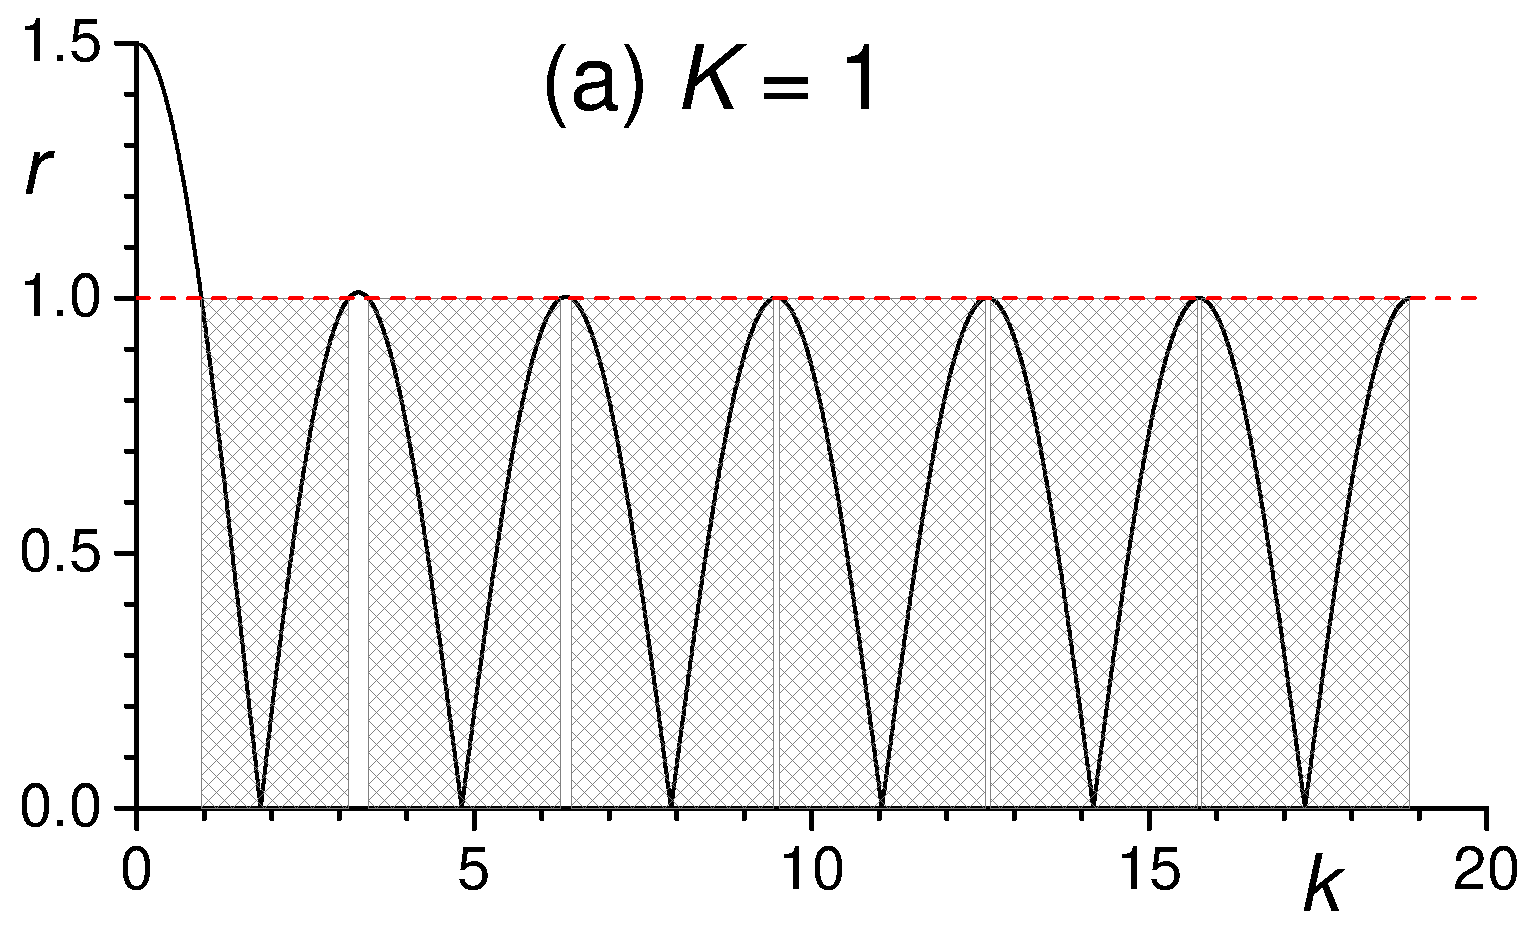
\epsfig{file=bandf1.eps,width=\linewidth}
            \end{subfigure}
            \hfill
            \begin{subfigure}{0.49\linewidth}
                \centering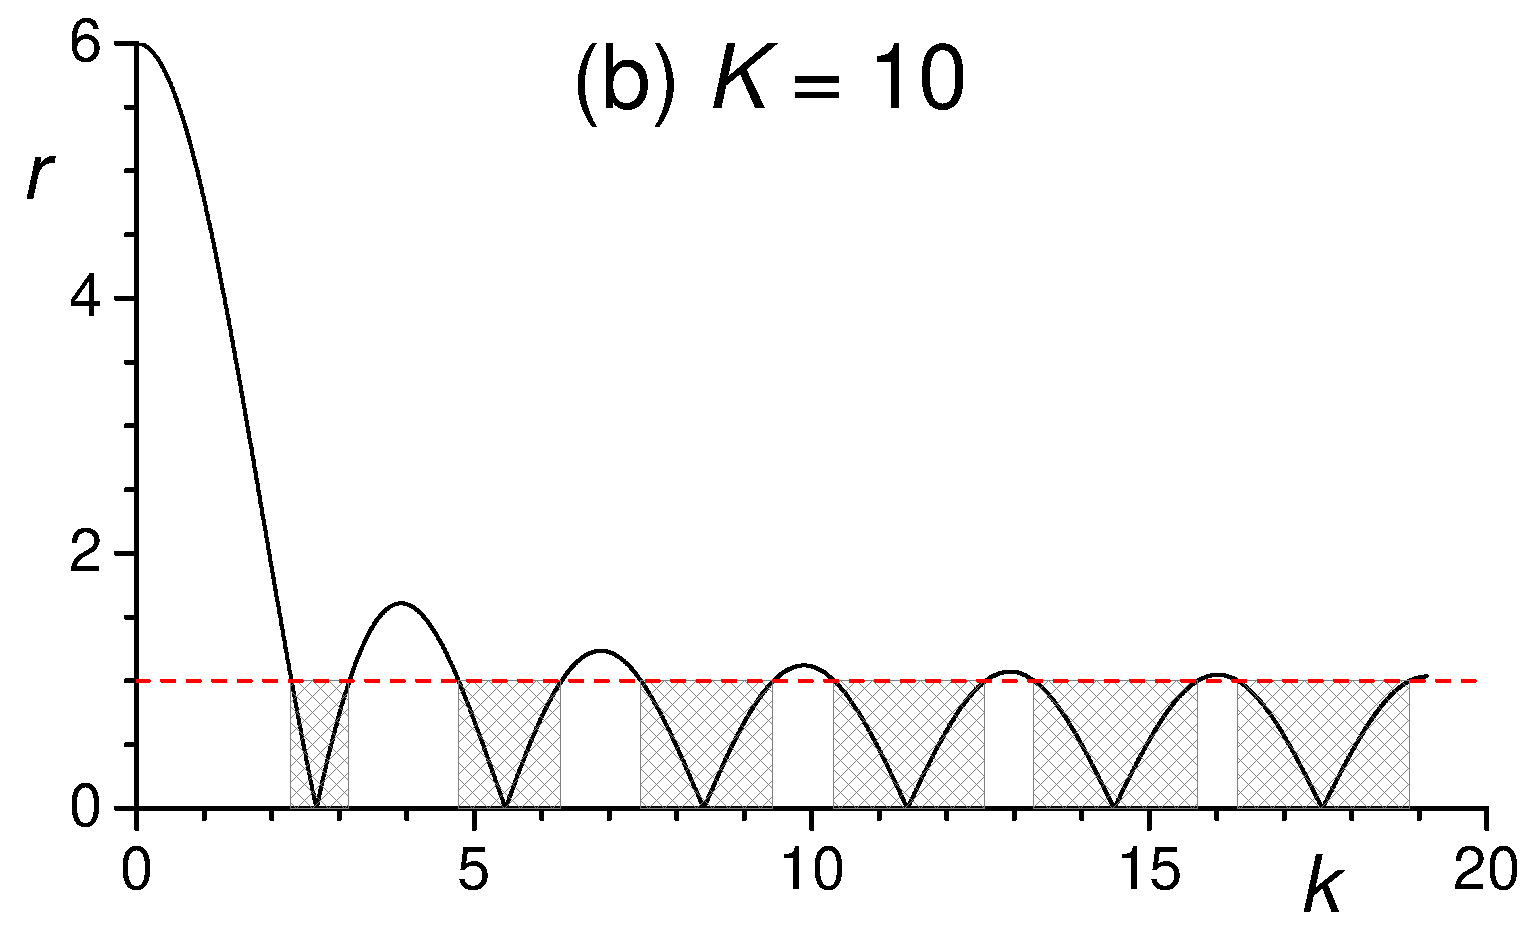
\epsfig{file=bandf10.eps,width=\linewidth}
            \end{subfigure}
			\scaption{
				Funkce $r$ (černá čára) pro dvě hodnoty parametru $K$ a mřížkovou konstantu $a=1$.
				Pásy, v nichž je splněna podmínka~\eqref{eq:DiracCombBandCondition} jsou vyznačeny šrafováním.
			}
			\label{fig:DiracCombBandCondition}
		\end{figure}

		Veličina $r$ je pro dvě hodnoty $K$ zakreslena na obrázku~\ref{fig:DiracCombBandCondition}.
		Několik pozorování:
		\begin{itemize}
		\item
			Pro $K\neq0$ má energetické spektrum ~\emph{pásovou strukturu:} povolené pásy $r\leq1$ střídají zakázané pásy $r>1$, viz obrázek~\ref{fig:DiracCombBandCondition}.
		
		\item
			Hodnota funkce $r$ pro $k=0$ je
			\begin{equation}
				r_{0}=\abs{1+\frac{Ka}{2}},
			\end{equation}
			tj. pokud $K>0$ nebo $K<-\frac{4}{a}$, je na nulové energii vždy zakázaný pás.
			
		\item
			Pro $K>0$ je horní hranice povoleného pásu vždy na hodnotě
			\begin{equation}\label{eq:DiracCombBandTop}
				ka=n\pi,\qquad n\in\mathbb{N}.
			\end{equation}
			Pásy lze tedy indexovat číslem $n$.

		\item
			Pokud $K=0$, jsou povolené všechny energie $E>0$.
			Řešení odpovídá pohybu volné částice.
			
		\item
			S rostoucí hodotou $K$ se pásy zužují a pro $K\rightarrow\infty$ se spektrum redukuje na čárové spektrum~\eqref{eq:DiracCombBandTop}, tj.
			\begin{equation}
				E_{n}=\frac{\hbar^{2}\pi^{2}}{2Ma^{2}}n^{2},
			\end{equation}
			což odpovídá spektru nekonečné hluboké jednorozměrné pravoúhlé jámy šířky $a$.
		\end{itemize}		

	\item
		\begin{figure}[!htbp]
            \begin{subfigure}{0.49\linewidth}
                \centering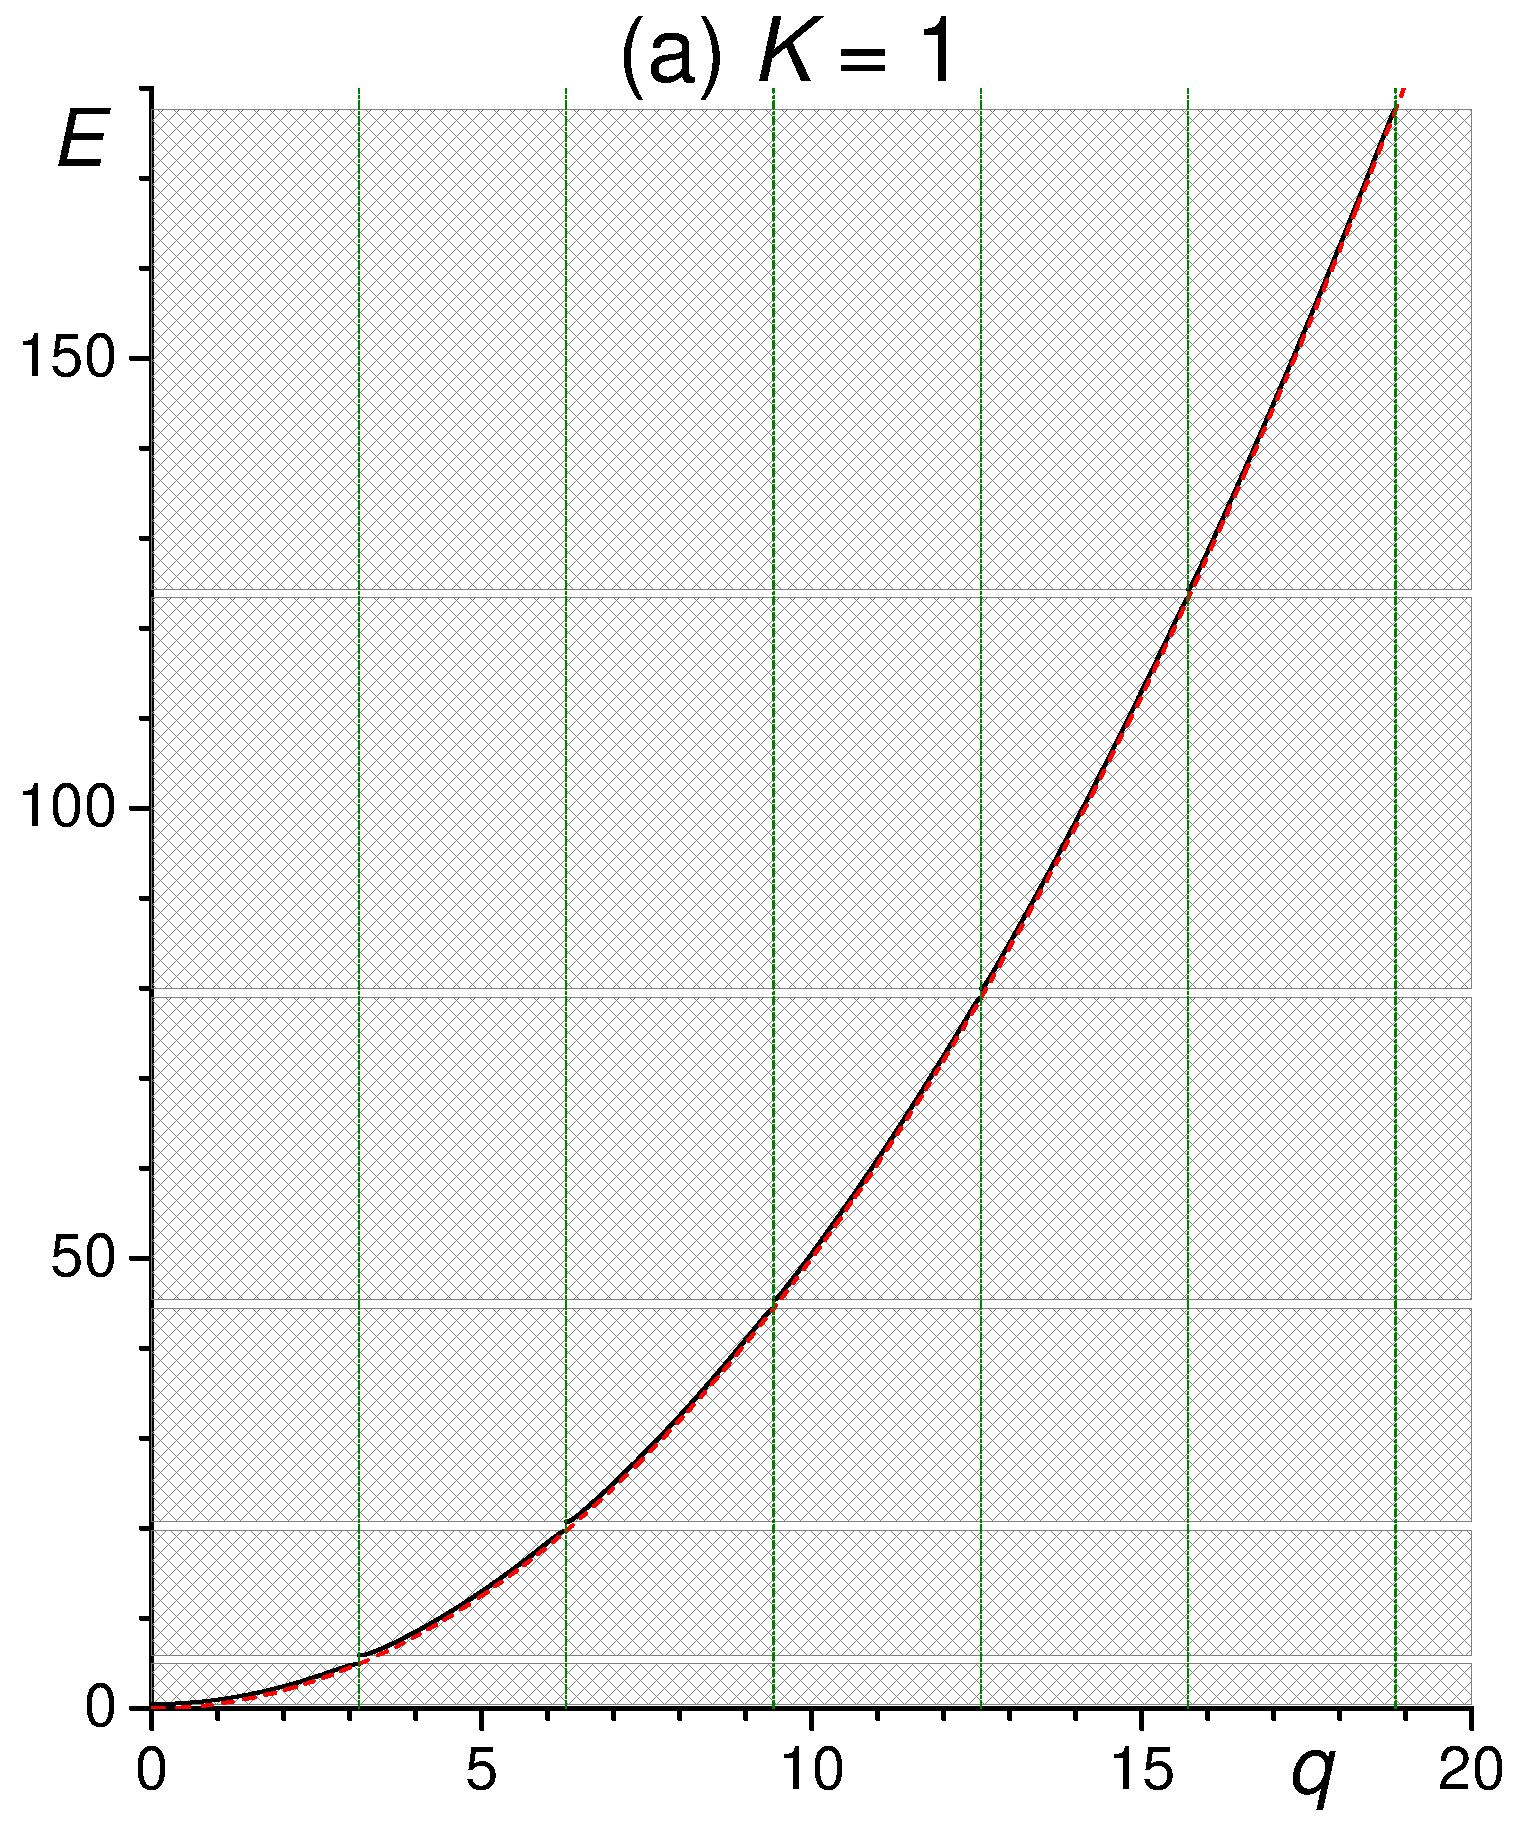
\epsfig{file=bands1.eps,width=\linewidth}
            \end{subfigure}
            \hfill
            \begin{subfigure}{0.49\linewidth}
                \centering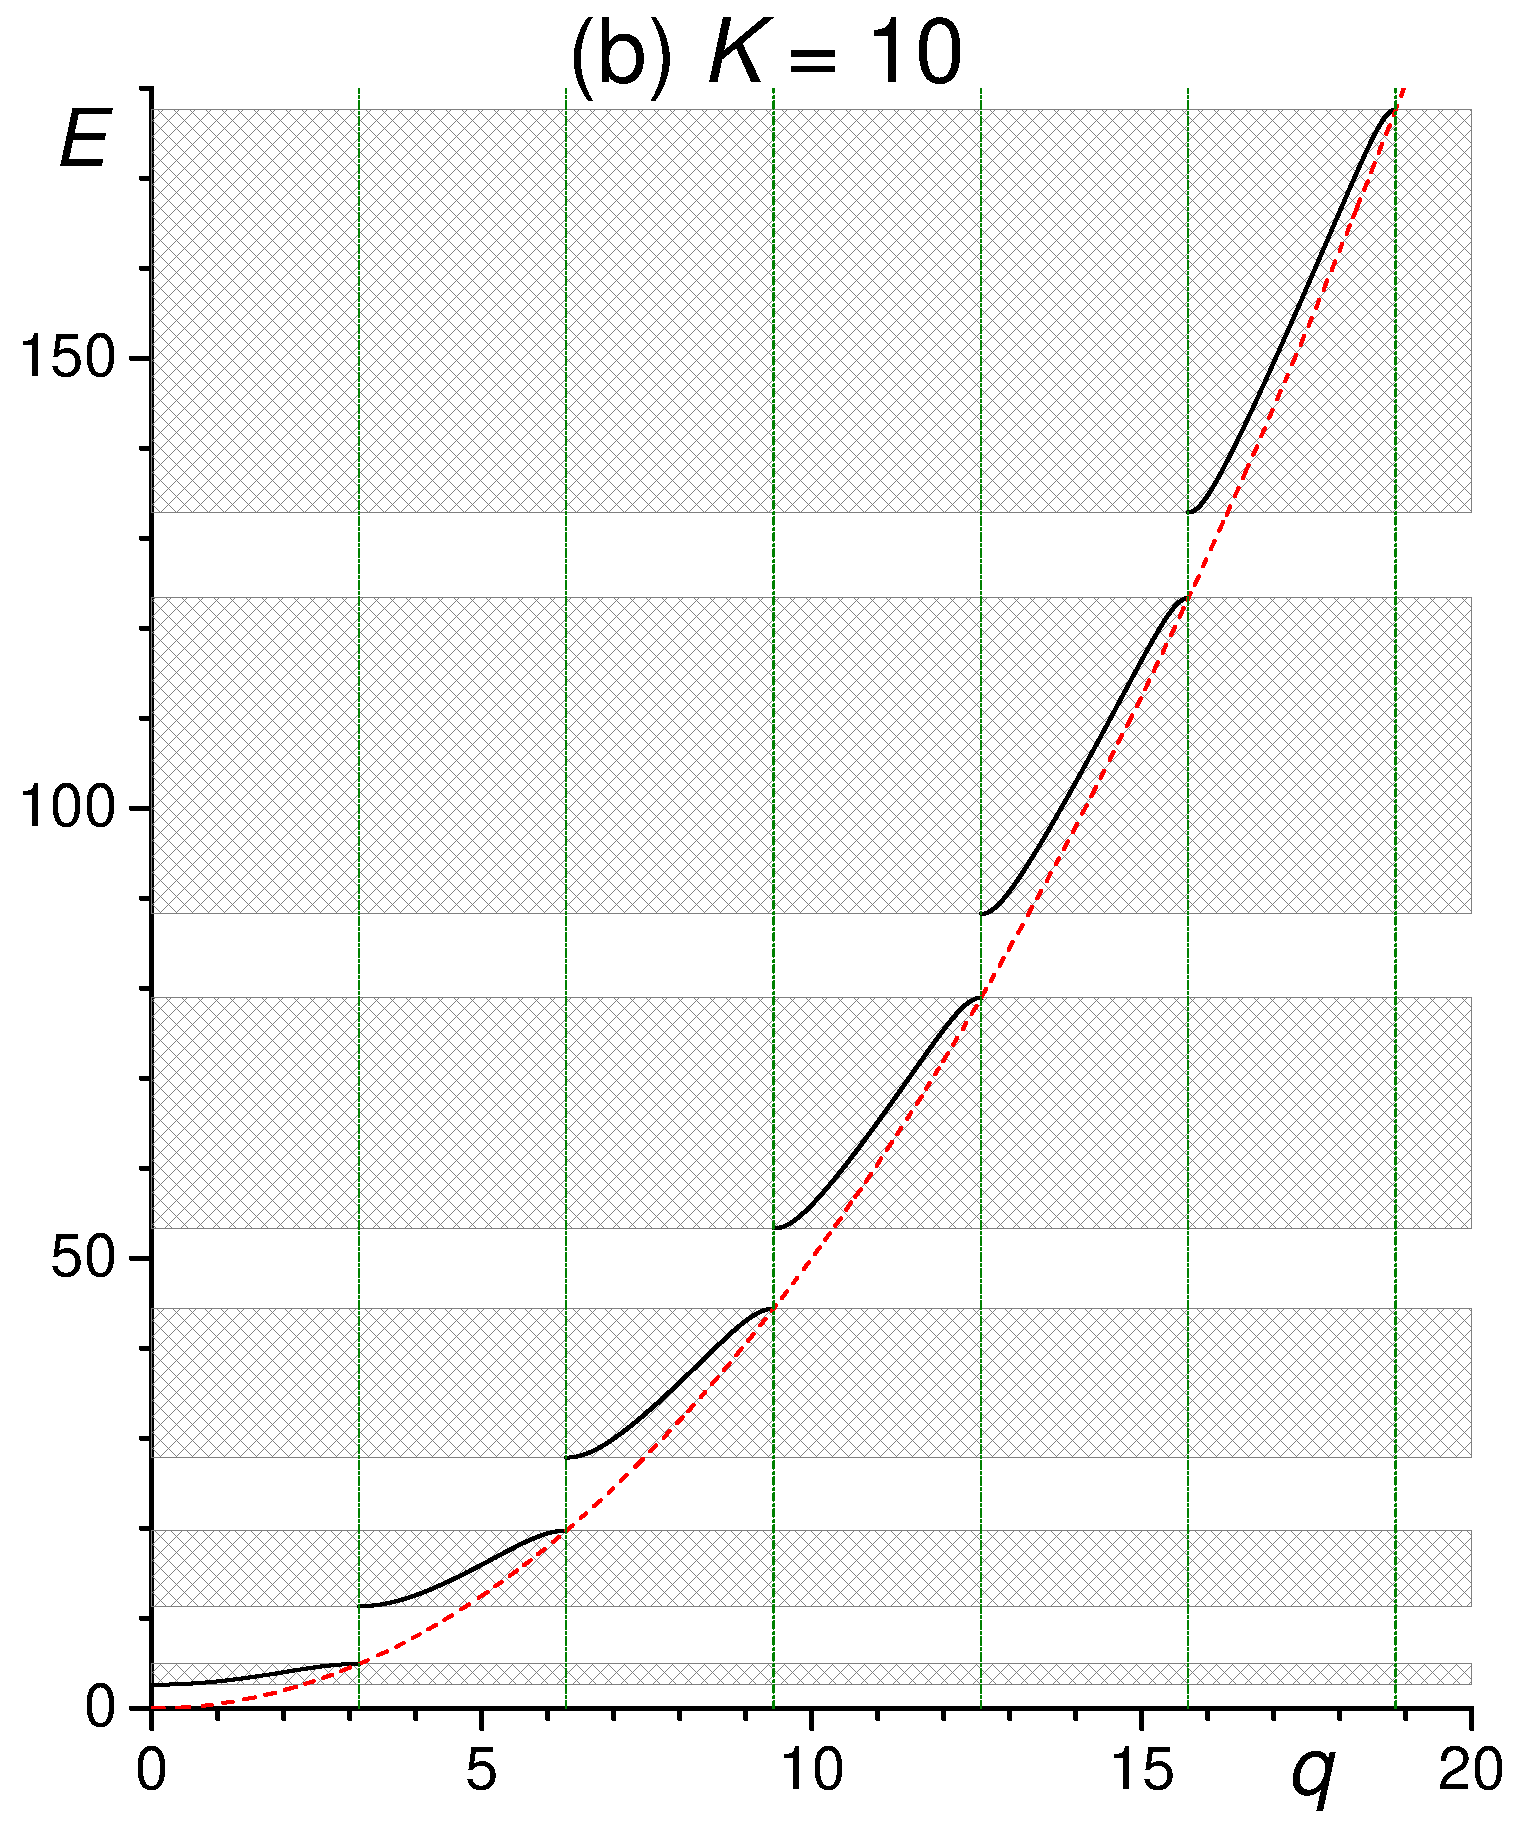
\epsfig{file=bands10.eps,width=\linewidth}
            \end{subfigure}
            \begin{subfigure}{0.49\linewidth}
                \centering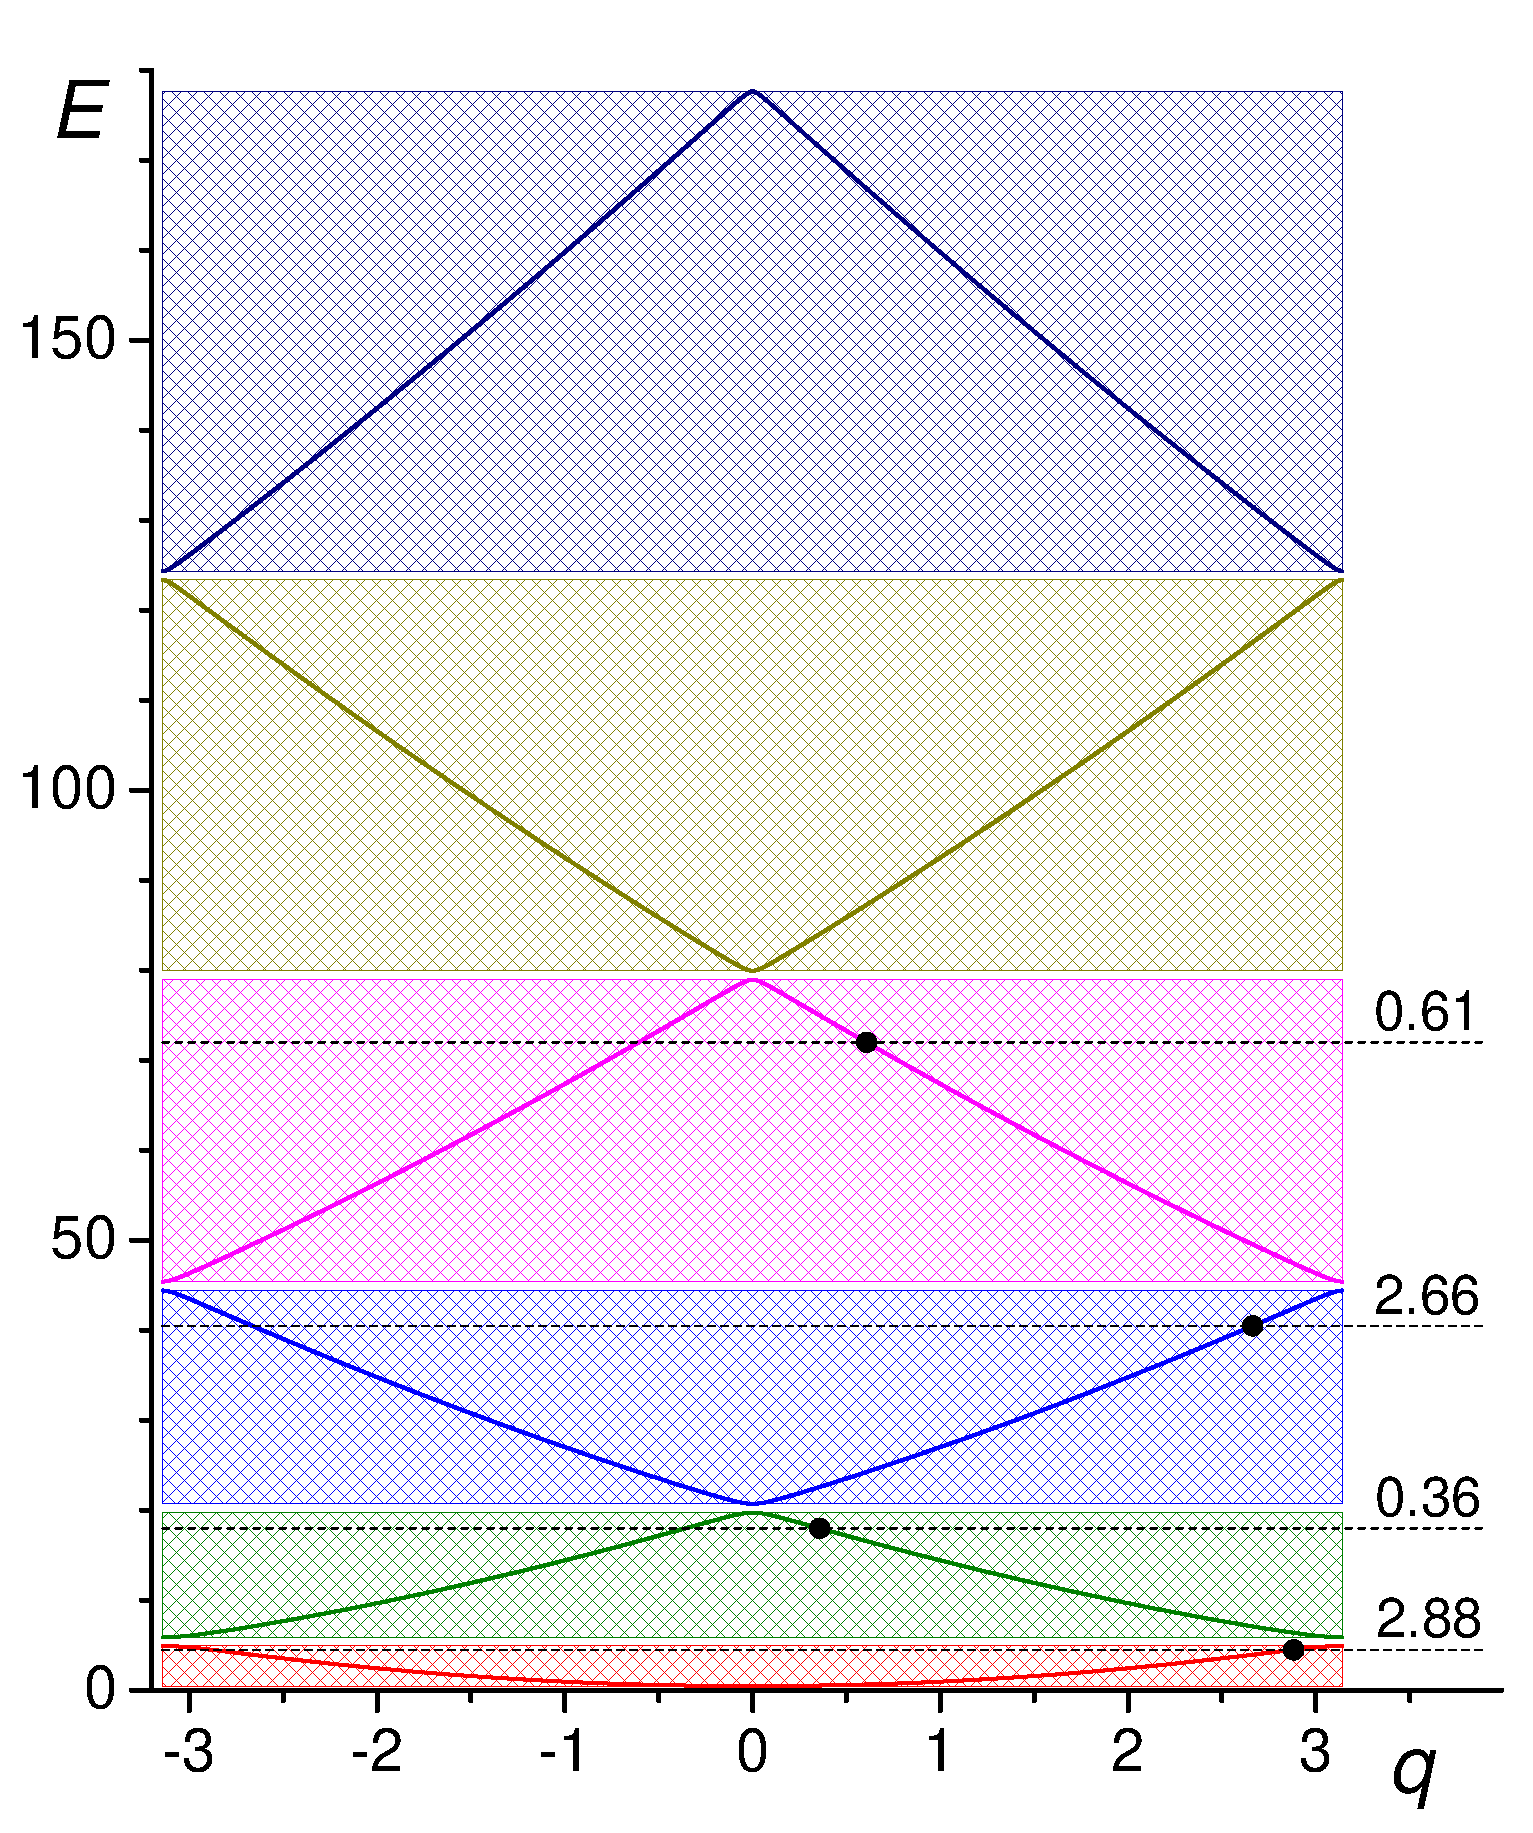
\epsfig{file=Brillouin1.eps,width=\linewidth}
            \end{subfigure}
            \hfill
            \begin{subfigure}{0.49\linewidth}
                \centering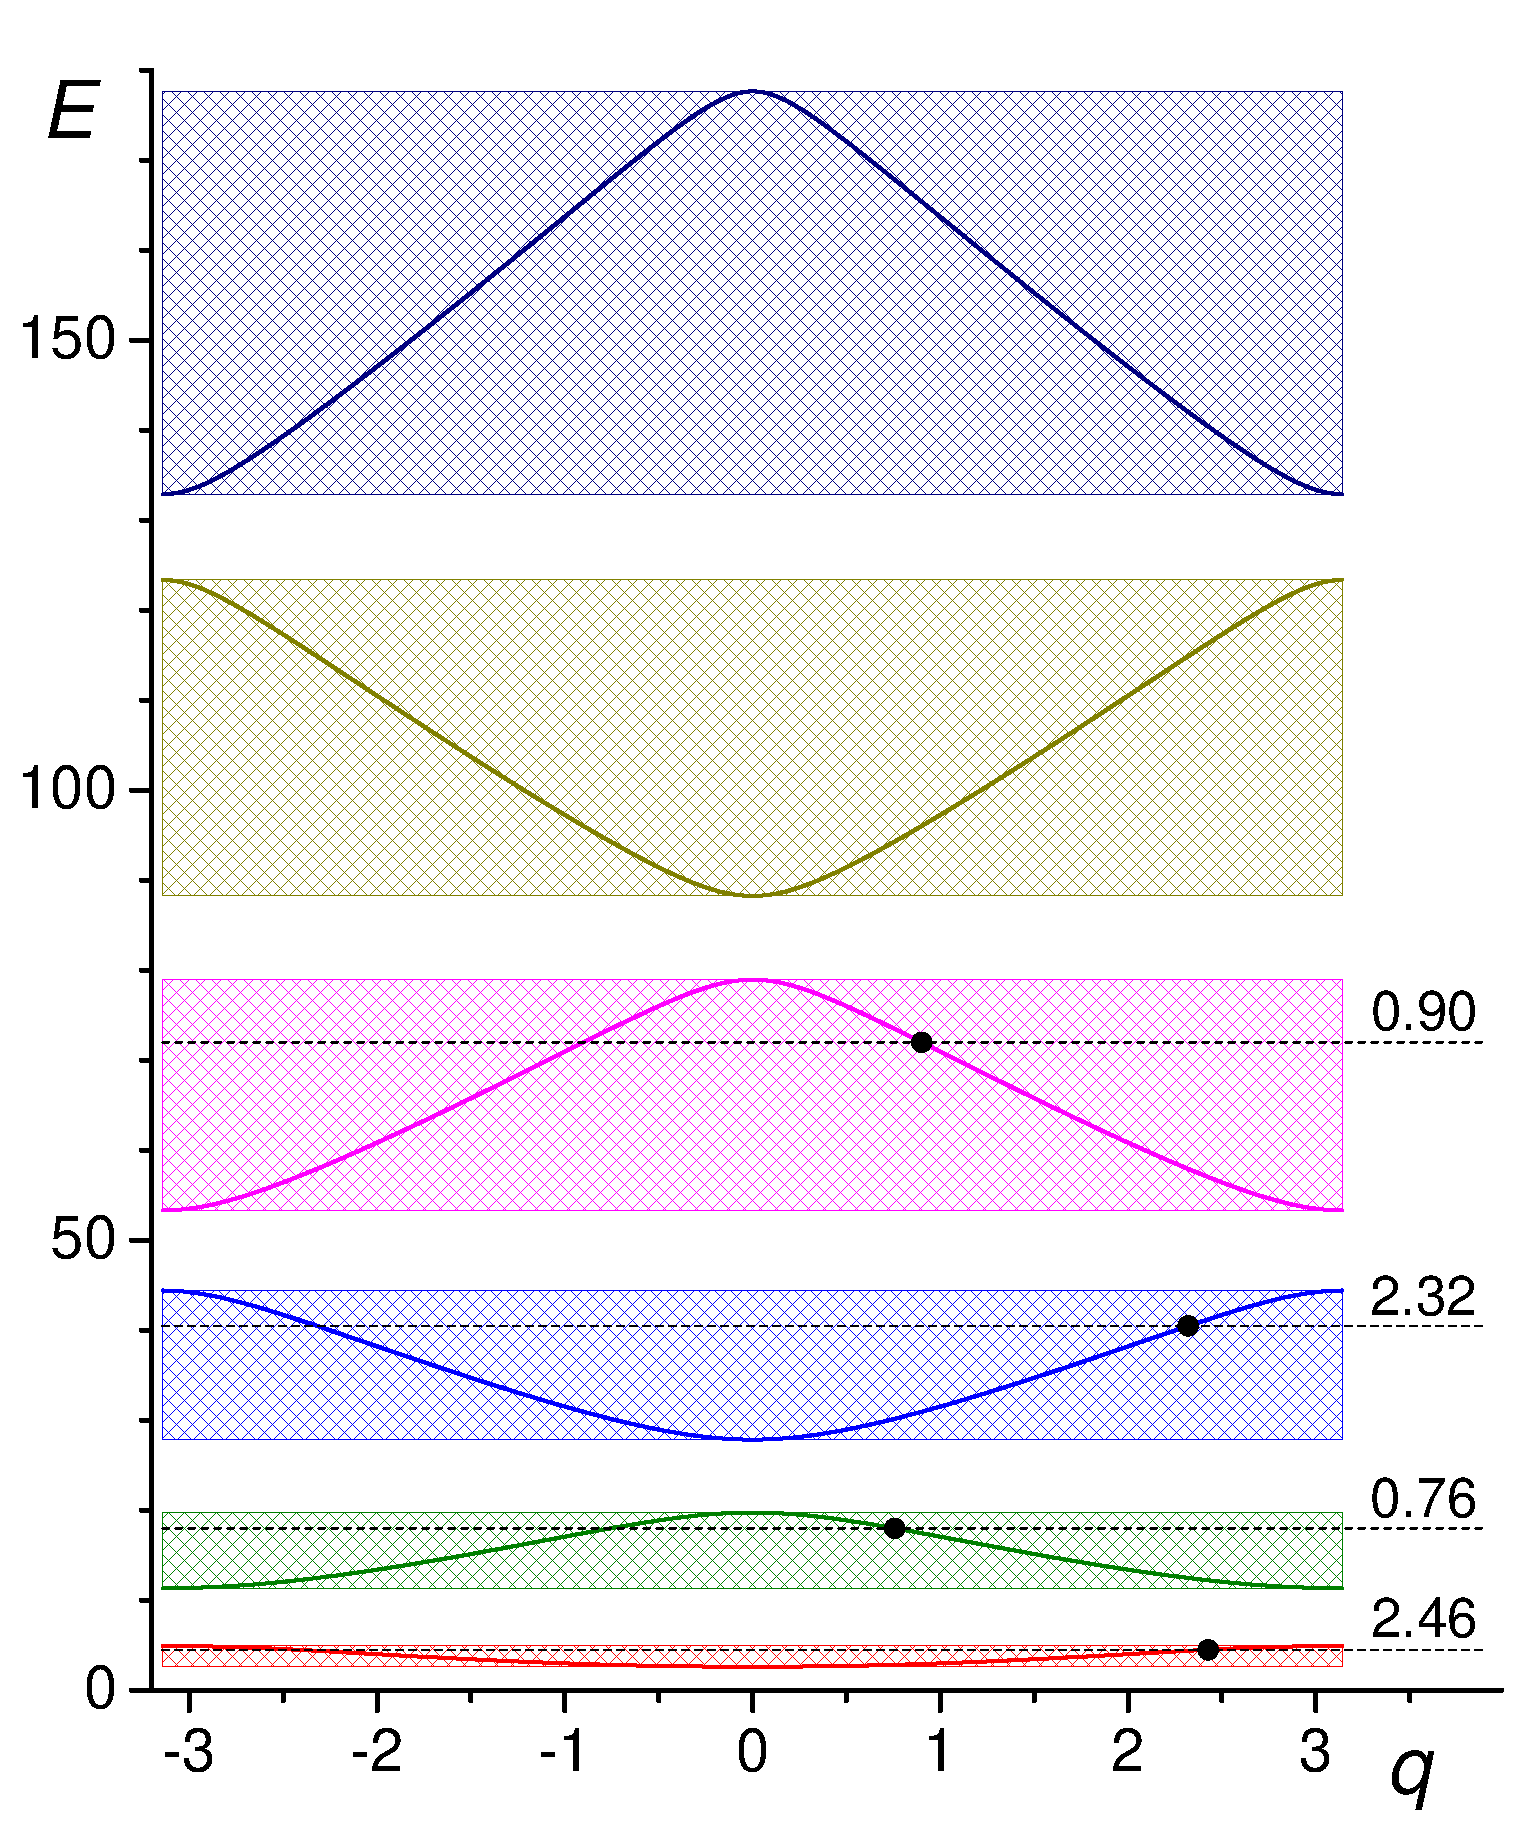
\epsfig{file=Brillouin10.eps,width=\linewidth}
            \end{subfigure}
			\scaption{
				\emph{1. řádek:} Disperzní relace v konvenci~\eqref{eq:DiracCombBandUnique} pro dvě hodnoty $K$ (černá čára).
				Červená čárkovaná čára odpovídá disperzní relaci pro volnou částici $E=\hbar^{2}q^{2}/(2M)$.
				Svislé zelené čerchované čáry vyznačují horní hranice pásů~\eqref{eq:DiracCombBandTop}.				
				Šrafováním jsou znázorněny povolené pásy.				
				\emph{2. řádek:}
				Disperzní relace pro 1. Brillouinovu zónu~\eqref{eq:Brillouin}.
				Jednotlivé pásy jsou znázorněny odlišnými barvami.
				Černými čárkovanými čarami jsou vyznačeny energie a vypsány hodnoty kvazihybnosti $q$ pro obrázek~\ref{fig:DiracCombWaveFunctions}.
			}
			\label{fig:DiracCombBands}
		\end{figure}

		Pokud rovnici~\eqref{eq:DiracCombBand} pro hodnotu $ka$ splňuje nějaké $qa$, pak ji stejně dobře splňuje $qa+2\pi m$, kde $m\in\mathbb{Z}$, přičemž vlnová funkce zůstane stejná.
		Jedna možná konvence znázornění výsledů tedy spočívá v tom, že se ke každé hodnotě $\pi n\leq ka\leq\pi(n+1)$ přidruží $qa$ tak, aby leželo v intervalu $\pi m\leq qa\leq\pi(m+1)$ pro $n=m$, tj.
        \begin{subequations}
            \begin{align}
                &\pi n\leq ka\leq\pi(n+1),\\
                &\pi n\leq qa\leq\pi(n+1),\qquad n\in\mathbb{N}.
            \end{align}
            \label{eq:DiracCombBandUnique}
        \end{subequations}
		Tímto způsobem je docíleno jednoznačného přiřazení $k\leftrightarrow q$.

		Druhá běžně používaná konvence omezuje hodnotu $q$ na tzv. \emph{1. Brillouinovu zónu},\index{zóna!Brillouinova} což je množina nejmenších $q$ takových, že dávají v daném pásu $n$ jednoznačně vlnovou funkci.
		Pro jednorozměrnou mřížku je 1. Brillouinova zóna interval
		\begin{equation}\label{eq:Brillouin}
			qa\in[-\pi,\pi].
		\end{equation}

        Disperzní relace $E=E(q)$ v obou konvencích je zobrazena na obrázku~\ref{fig:DiracCombBands}.
		
		\begin{figure}[!htbp]
            \begin{subfigure}{0.49\linewidth}
                \centering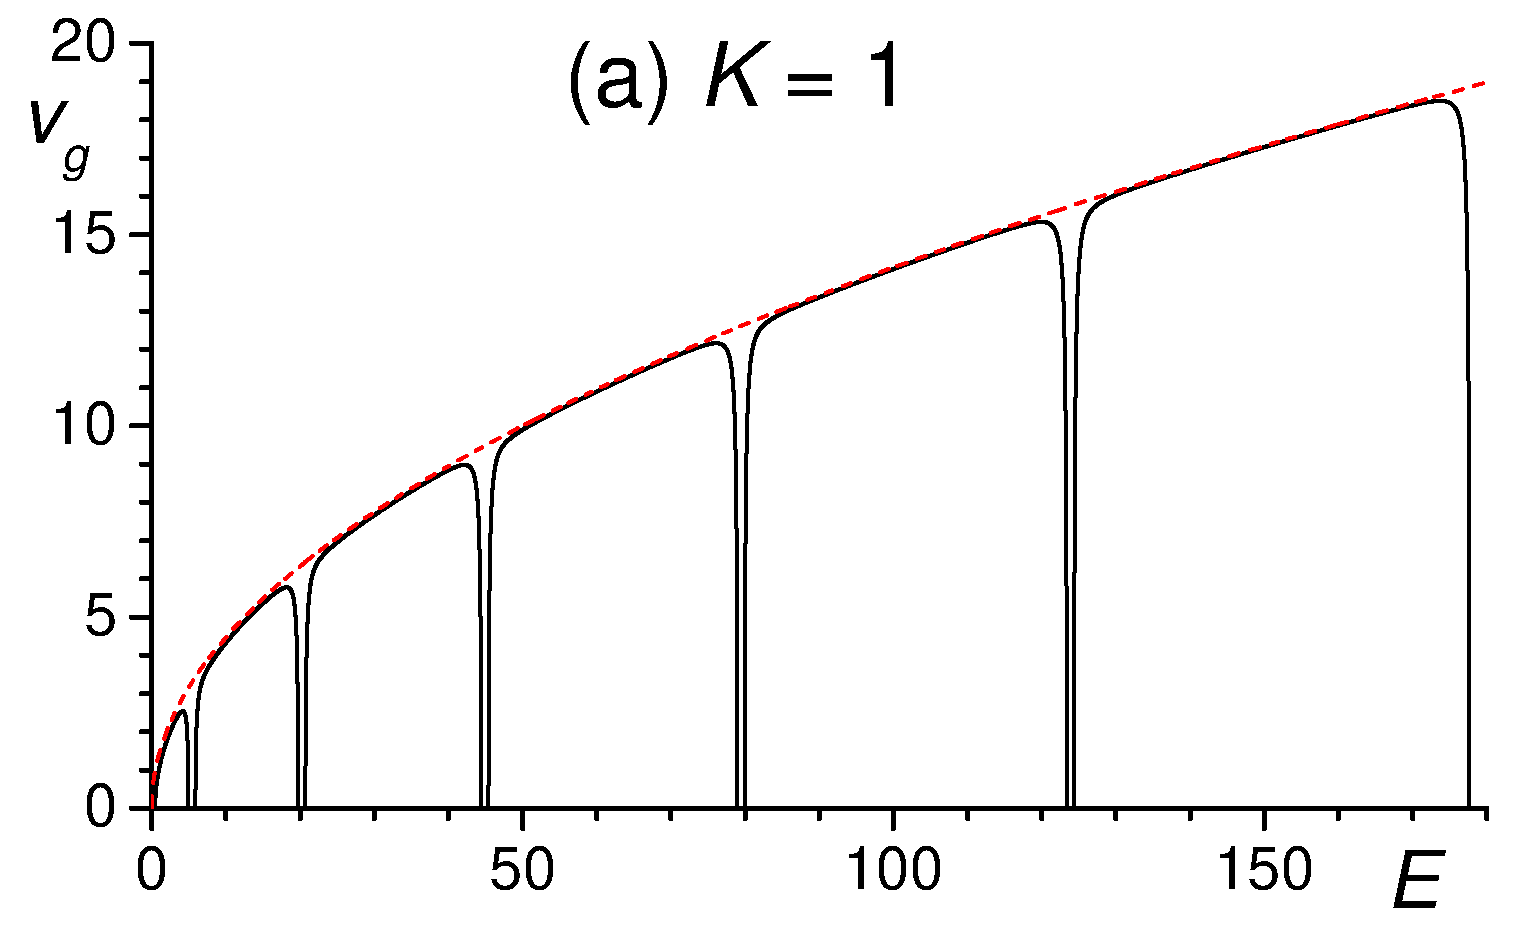
\epsfig{file=vgE1.eps,width=\linewidth}
            \end{subfigure}
            \hfill
            \begin{subfigure}{0.49\linewidth}
                \centering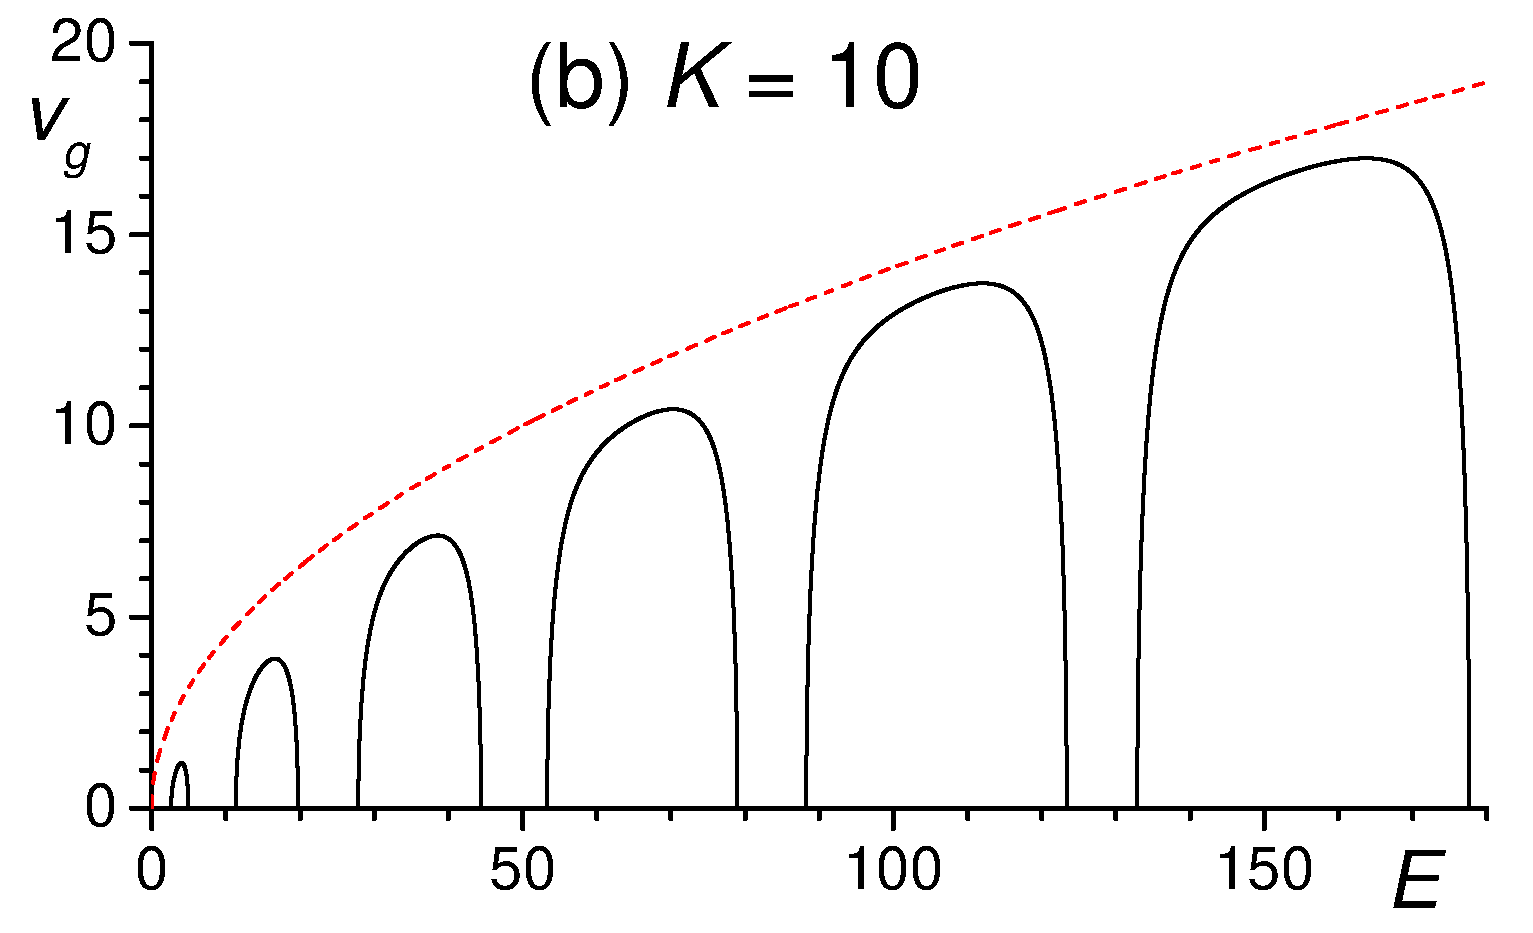
\epsfig{file=vgE10.eps,width=\linewidth}
            \end{subfigure}
            \begin{subfigure}{0.49\linewidth}
                \centering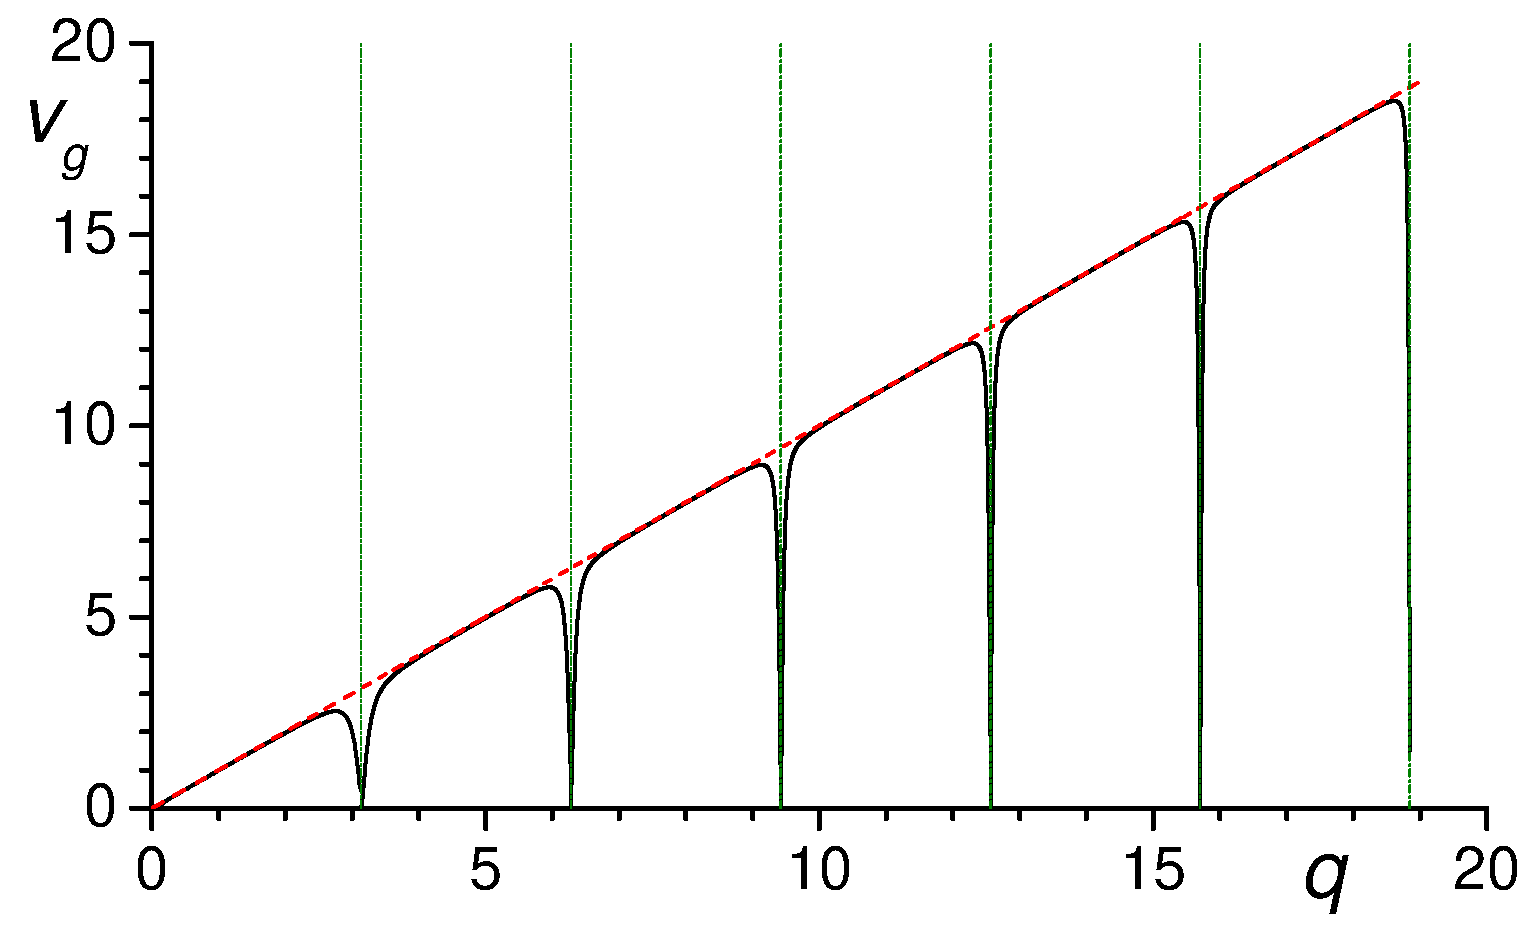
\epsfig{file=vgq1.eps,width=\linewidth}
            \end{subfigure}
            \hfill
            \begin{subfigure}{0.49\linewidth}
                \centering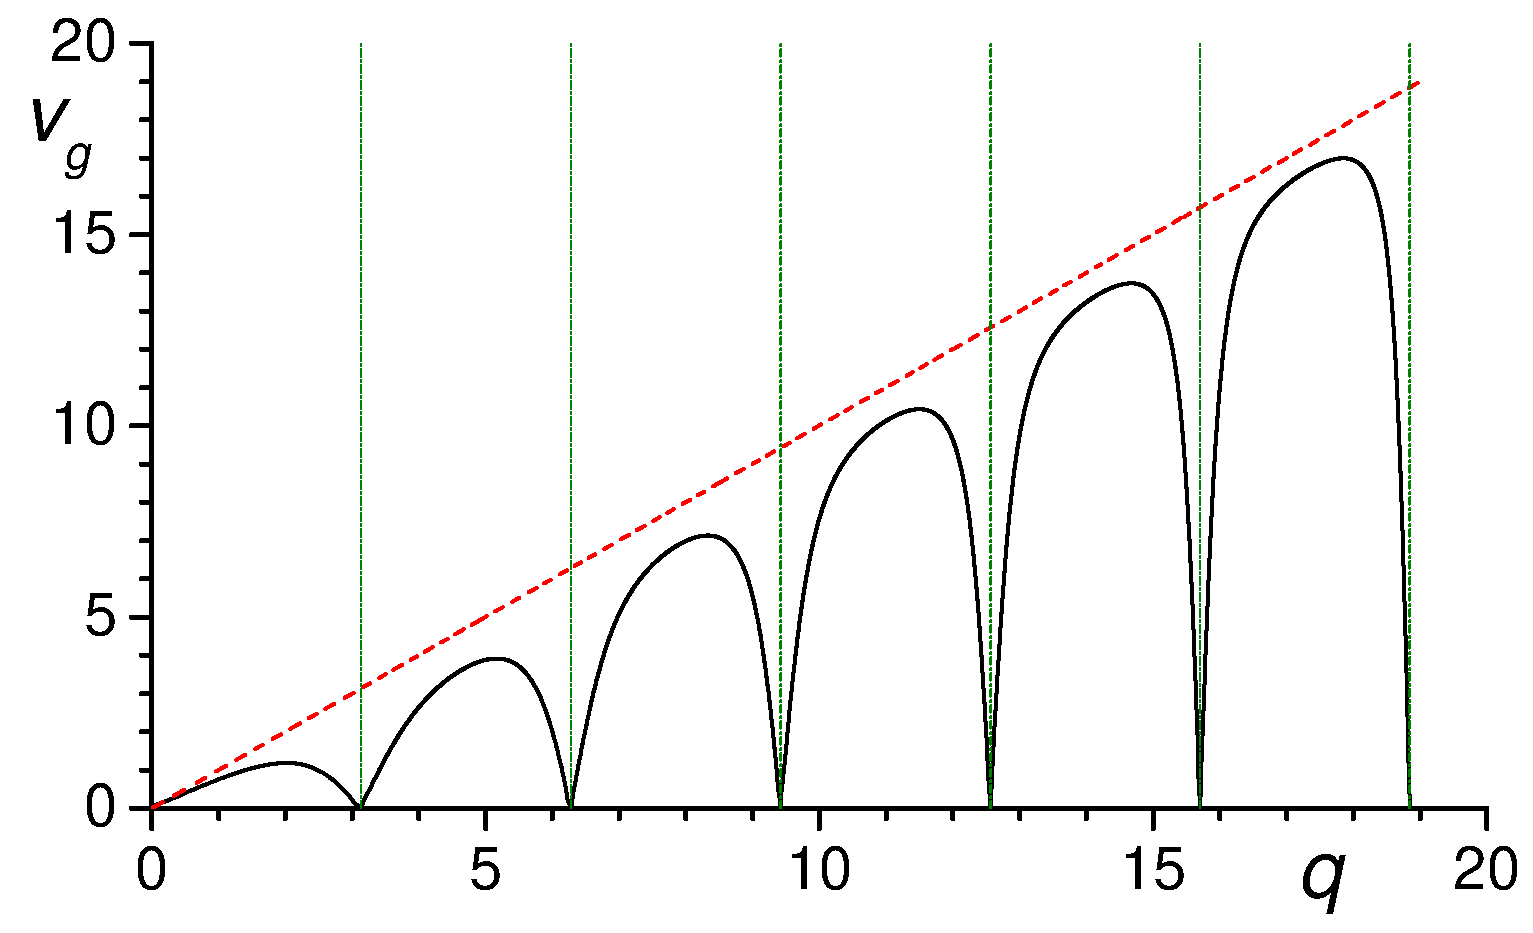
\epsfig{file=vgq10.eps,width=\linewidth}
            \end{subfigure}
			\scaption{
				Grupová rychlost~\eqref{eq:DiracCombGroupVelocity} v závislosti na energii (1. řádek) a na kvazihybnosti (2. řádek).
				Ve 2. řádku jsou hranice pásů $q=\pi n$ znázorněny svislými zelenými čerchovanými čarami.
				Červená čárkovaná čára odpovídá rychosti pro volnou částici $E=\hbar q/M$.
			}
			\label{fig:DiracCombGroupVelocity}
		\end{figure}

        \begin{note}
            V 1. Brillouinově zóně musí mít Schrödingerova rovnice dvě lineárně nezávislá řešení.
            Druhé řešení získáme komplexním sdružením $\psi_{q}(x)\mapsto\psi_{q}^{*}(x)=\psi_{-q}(x)$.
            Tato vlnová funkce odpovídá opačné hodnotě kvazihybnosti.
        \end{note}
    
    \item
		Grupová rychost je zakreslena na obrázku~\ref{fig:DiracCombGroupVelocity}.
		Pro $q$ v blízkosti hranice pásu klesá rychost k nule.						

    \item
        Ze sešívací podmínky na spojitost vlnové funkce~\eqref{eq:DiracCombSew} plyne
        \begin{equation}
            A\left[1-\e^{-\im q a}\e^{\im k a}\right]=-B\left[1-\e^{-\im q a}\e^{-\im k a}\right],
        \end{equation}
        což dává vztah mezi konstantami $A$ a $B$:
        \begin{subequations}
            \begin{align}
                A&=-B\,\frac{1-\e^{-\im q a}\e^{-\im k a}}{1-\e^{-\im q a}\e^{\im k a}}
                =B\,\frac{\cos{qa}-\cos{ka}}{1-\cos{(q-k)a}}\e^{-\im k a},\\
                B&=-A\,\frac{1-\e^{-\im q a}\e^{\im k a}}{1-\e^{-\im q a}\e^{-\im k a}}
                =B\,\frac{\cos{qa}-\cos{ka}}{1-\cos{(q+k)a}}\e^{\im k a}.
            \end{align}
        \end{subequations}

        Integrace vlnové funkce na intervalu $[0,a]$~\eqref{eq:DiracCombWaveFunctionNormalization} dá podmínku
        \begin{align}
            1&=\int_{0}^{a}\left(A\e^{\im kx}+B\e^{-\im kx}\right)\left(A^{*}\e^{-\im kx}+B^{*}\e^{\im kx}\right)\d x\nonumber\\
             &=\int_{0}^{a}\left(\abs{A}^{2}+\abs{B}^{2}+AB^{*}\e^{2\im kx}+A^{*}B\e^{-2\im kx}\right)\d x\nonumber\\
             &=\left(\abs{A}^{2}+\abs{B}^{2}\right)a+\frac{1}{2\im k}\left[AB^{*}\left(\e^{2\im ka}-1\right)+A^{*}B\left(1-\e^{-2\im ka}\right)\right].
        \end{align}
        Spojení posledních dvou vztahů vede k výrazům
        \begin{align}
            1&=a\abs{B}^{2}\bigg\{1+\left[\frac{\cos{qa}-\cos{ka}}{1-\cos{(q-k)a}}\right]^{2}
                +\underbrace{\frac{2\sin{ka}}{ka}}_{\frac{4}{Ka}\left(\cos{qa}-\cos{ka}\right)}\frac{\cos{qa}-\cos{ka}}{1-\cos{(q-k)a}}\bigg\}\nonumber\\
             &=2a\abs{B}^{2}\frac{1-\cos{qa}\cos{ka}+\frac{2}{Ka}\left(\cos{qa}-\cos{ka}\right)^{2}}{1-\cos{(q-k)a}},
        \end{align}
        kde bylo využito vztahu~\eqref{eq:DiracCombBand} a první dva členy byly upraveny podle vzorců pro goniometrické funkce:
        \begin{align}
            1+\left[\frac{\cos{qa}-\cos{ka}}{1-\cos{(q-k)a}}\right]^{2}
                &=1+\left[\frac{-2\sin{\frac{q-k}{2}a}\,\sin{\frac{q+k}{2}a}}{2\sin^{2}\frac{q-k}{2}a}\right]^{2}\nonumber\\
                &=\frac{\sin^{2}{\frac{q-k}{2}a}+\sin^{2}{\frac{q+k}{2}a}}{\sin^{2}{\frac{q-k}{2}a}}\nonumber\\
                &=\frac{1-\cos{(q-k)a}+1-\cos{(q+k)a}}{1-\cos{(q-k)a}}\nonumber\\
                &=\frac{2-2\cos{qa}\cos{ka}}{1-\cos{(q-k)a}}.
        \end{align}
        
        \begin{figure}[!htbp]
            \begin{subfigure}{0.49\linewidth}
                \centering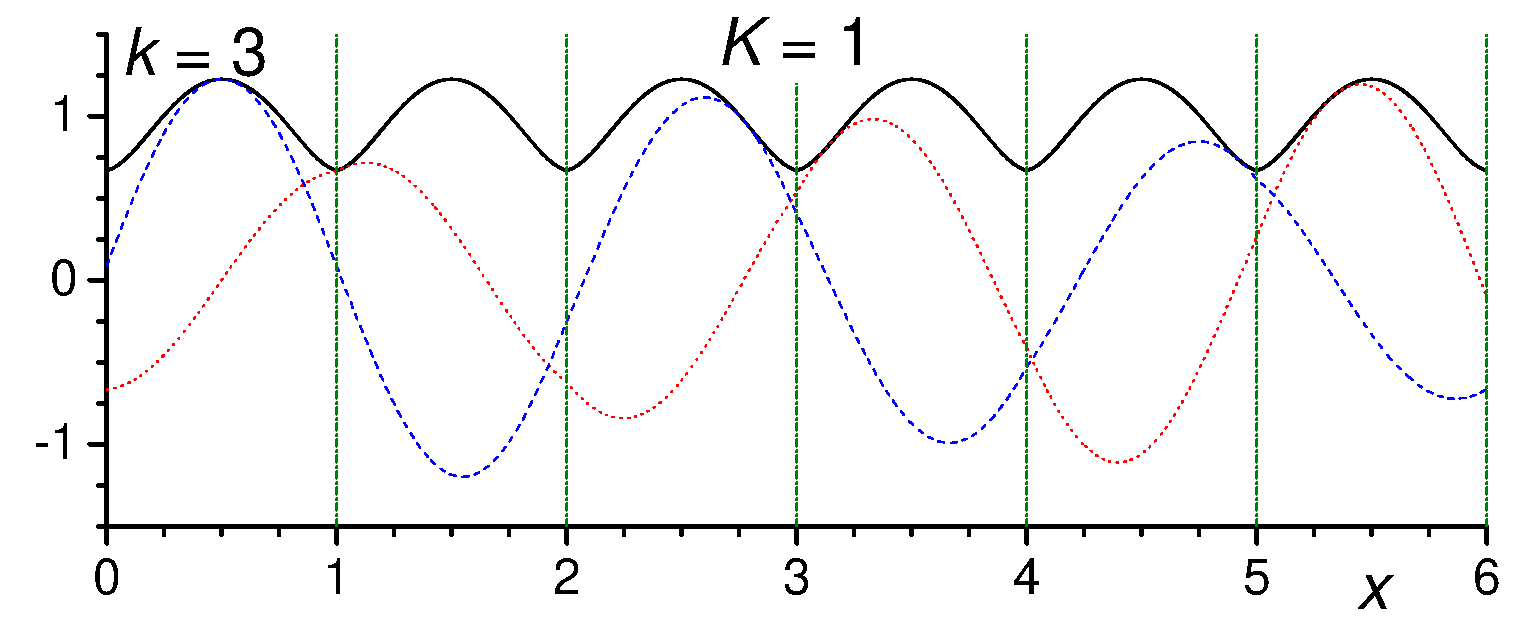
\epsfig{file=psi1_3.eps,width=\linewidth}
            \end{subfigure}
            \hfill
            \begin{subfigure}{0.49\linewidth}
                \centering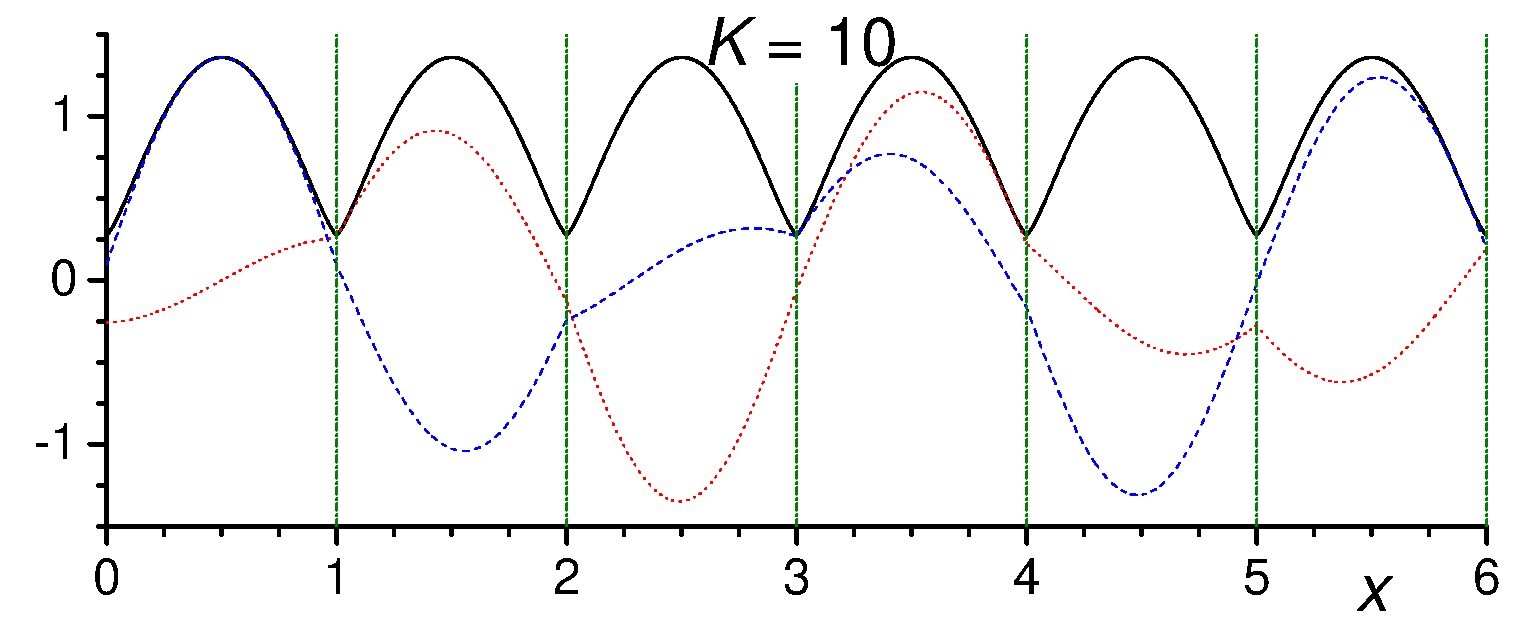
\epsfig{file=psi10_3.eps,width=\linewidth}
            \end{subfigure}
            \begin{subfigure}{0.49\linewidth}
                \centering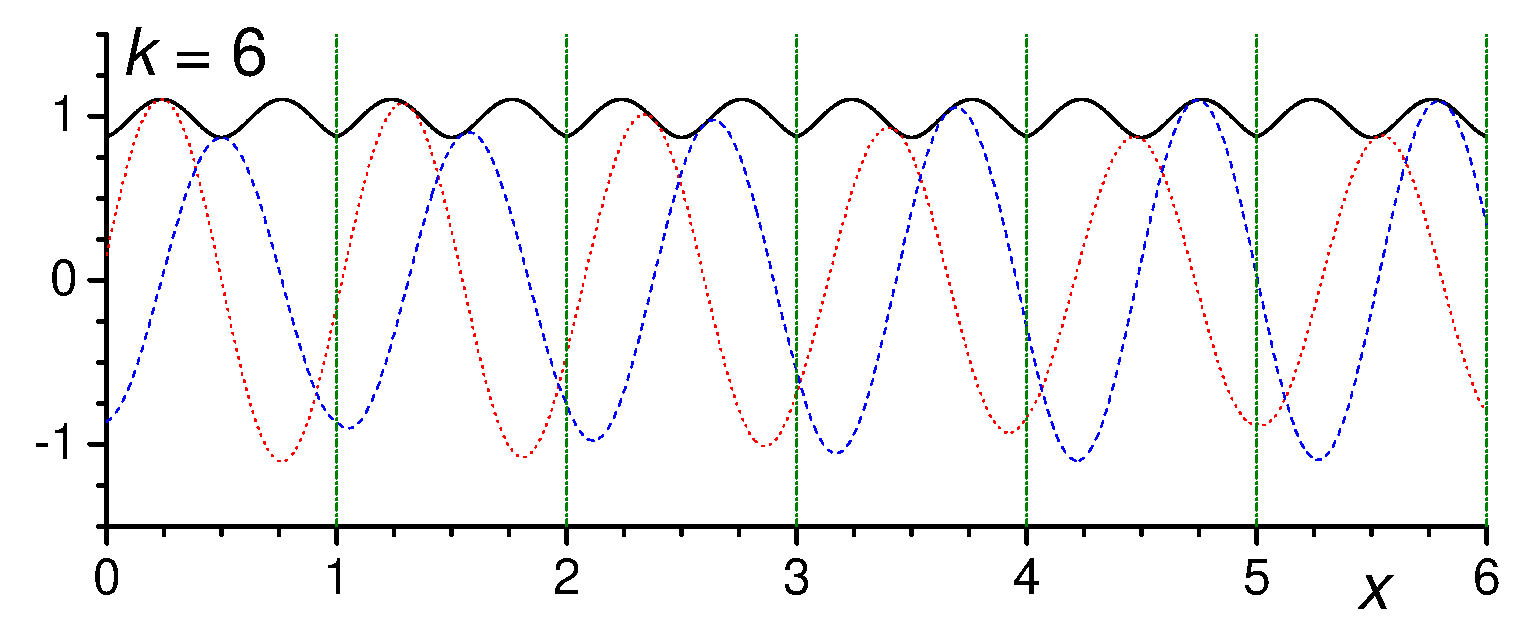
\epsfig{file=psi1_6.eps,width=\linewidth}
            \end{subfigure}
            \hfill
            \begin{subfigure}{0.49\linewidth}
                \centering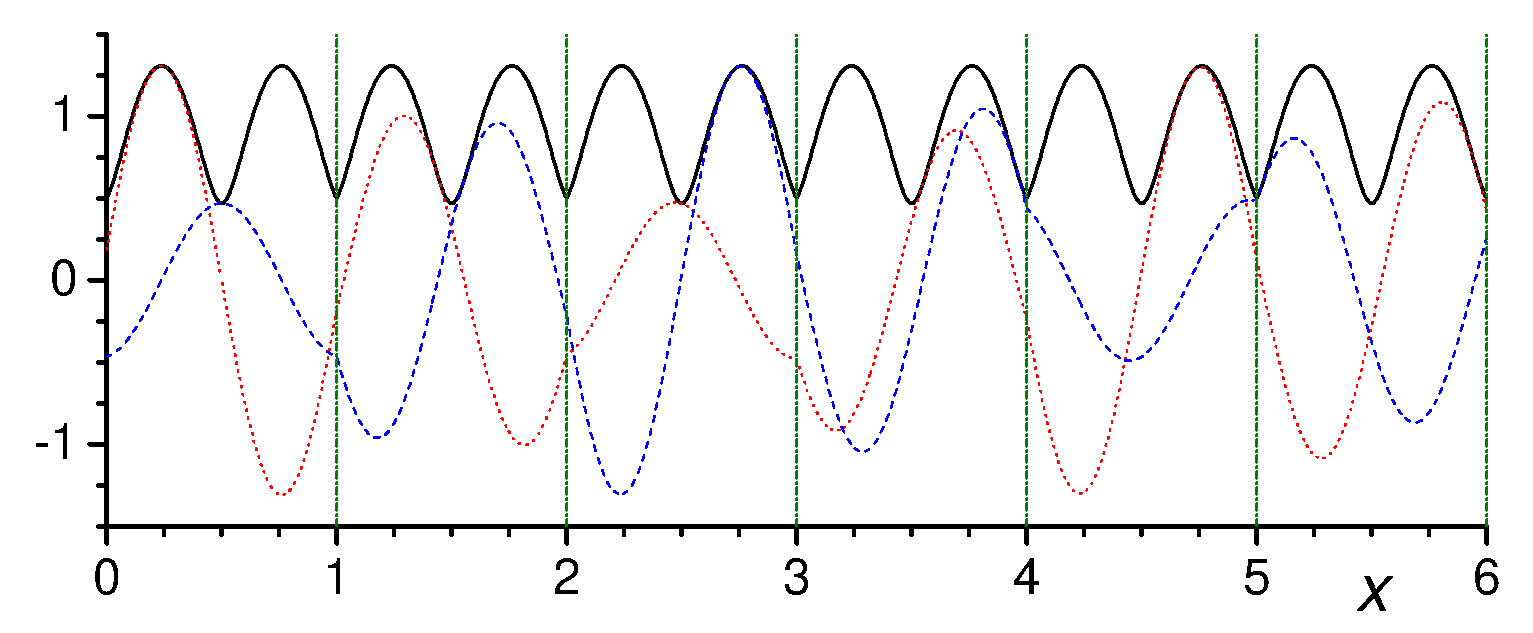
\epsfig{file=psi10_6.eps,width=\linewidth}
            \end{subfigure}
            \begin{subfigure}{0.49\linewidth}
                \centering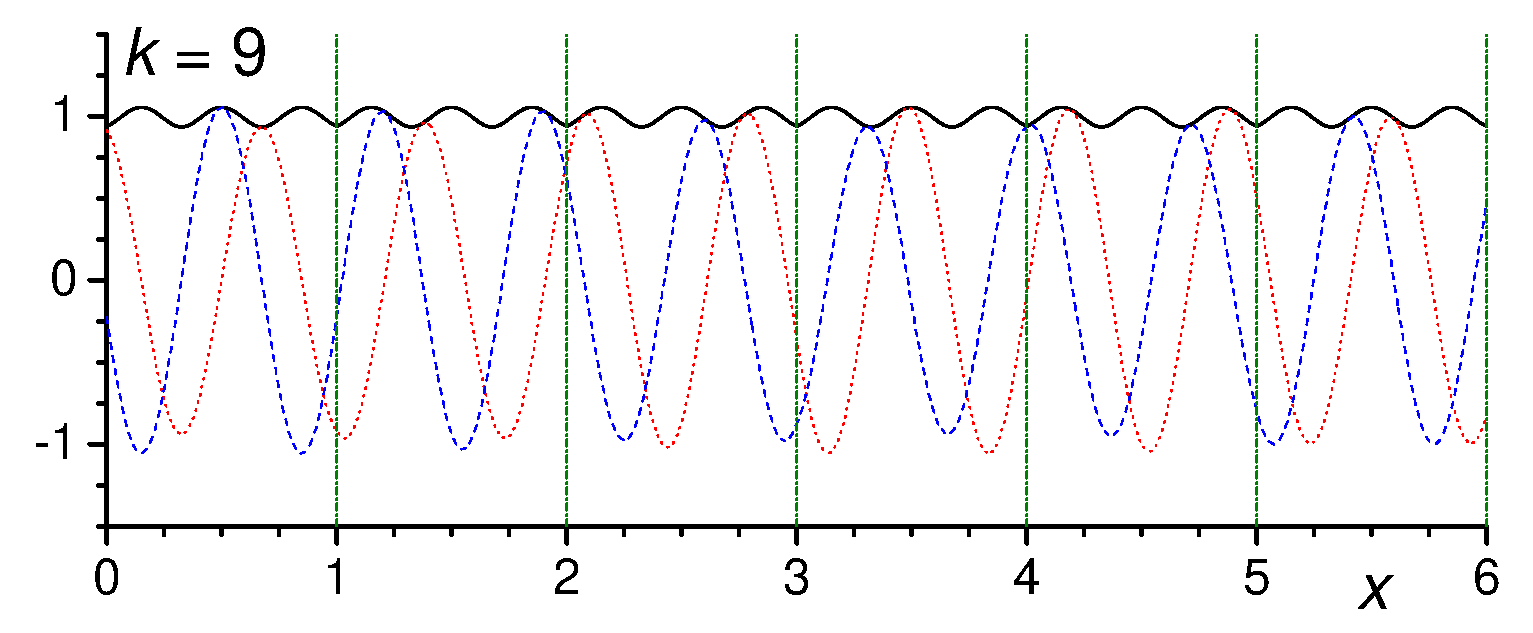
\epsfig{file=psi1_9.eps,width=\linewidth}
            \end{subfigure}
            \hfill
            \begin{subfigure}{0.49\linewidth}
                \centering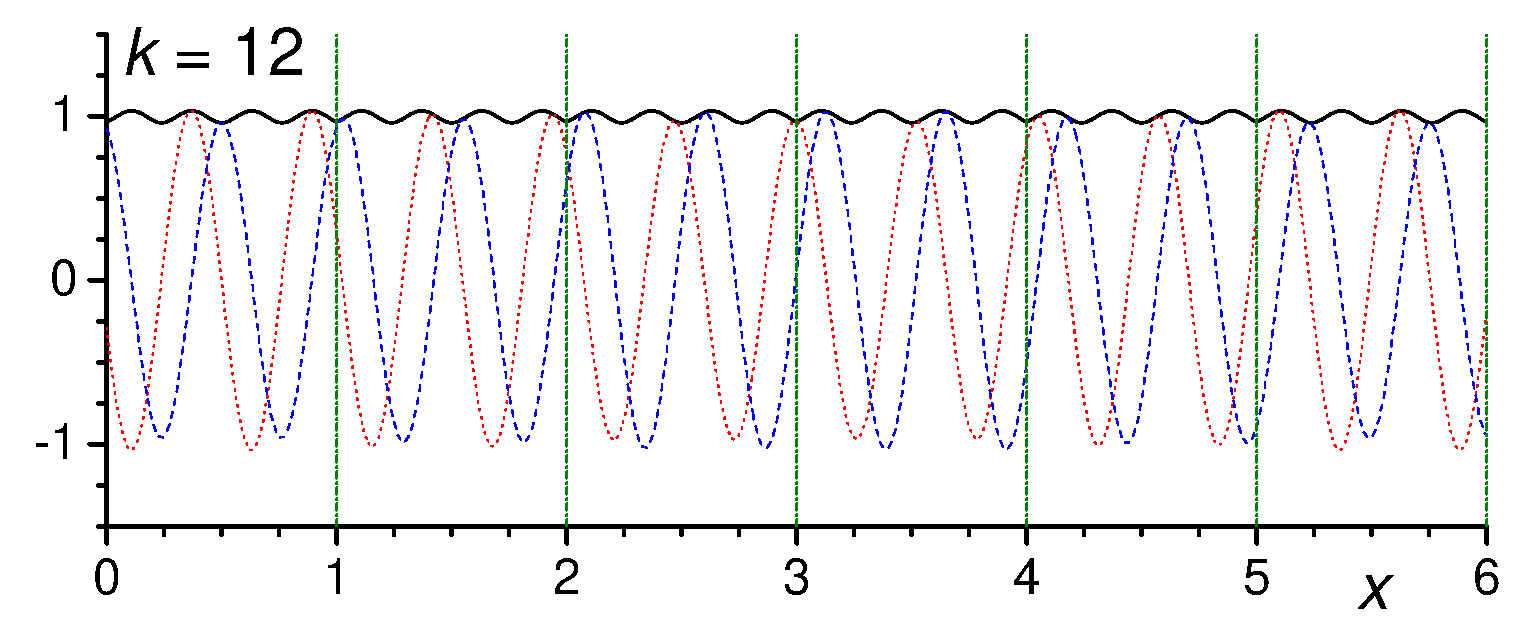
\epsfig{file=psi1_12.eps,width=\linewidth}
            \end{subfigure}
            \begin{subfigure}{0.49\linewidth}
                \centering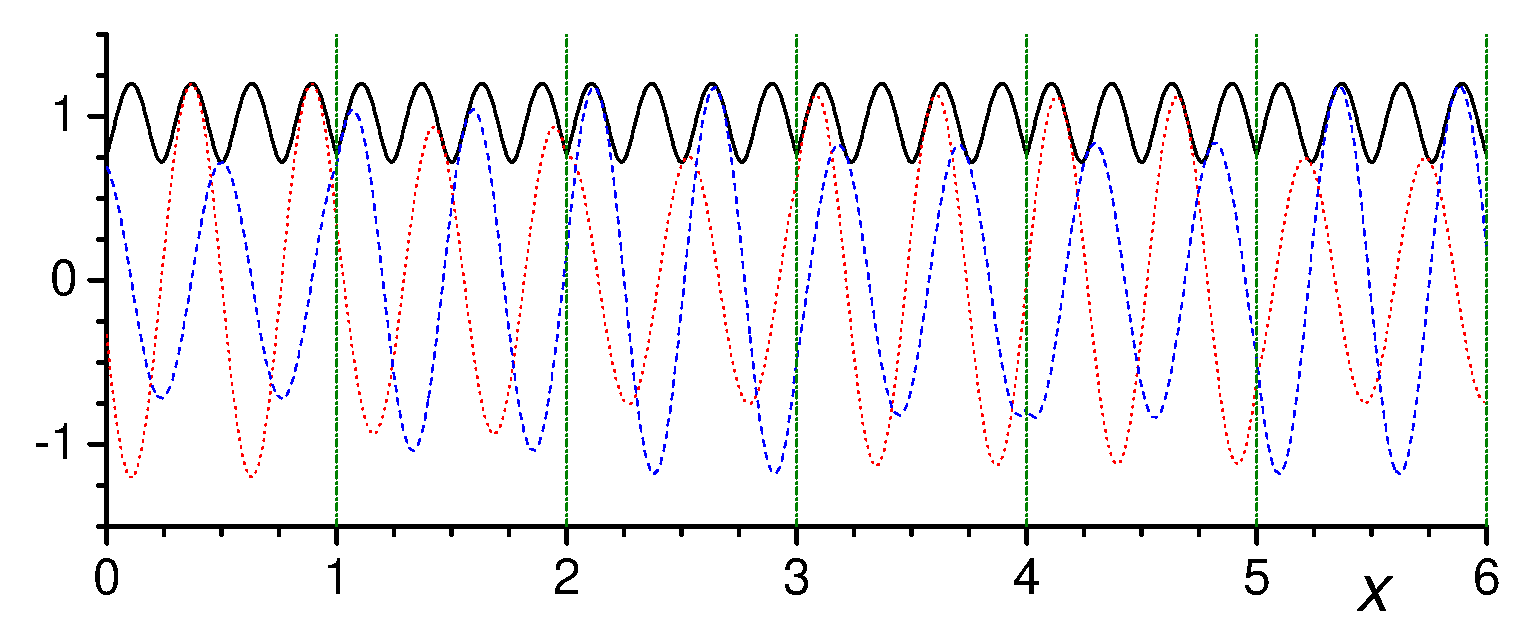
\epsfig{file=psi10_12.eps,width=\linewidth}
            \end{subfigure}
            \hfill
            \begin{subfigure}{0.49\linewidth}
                \centering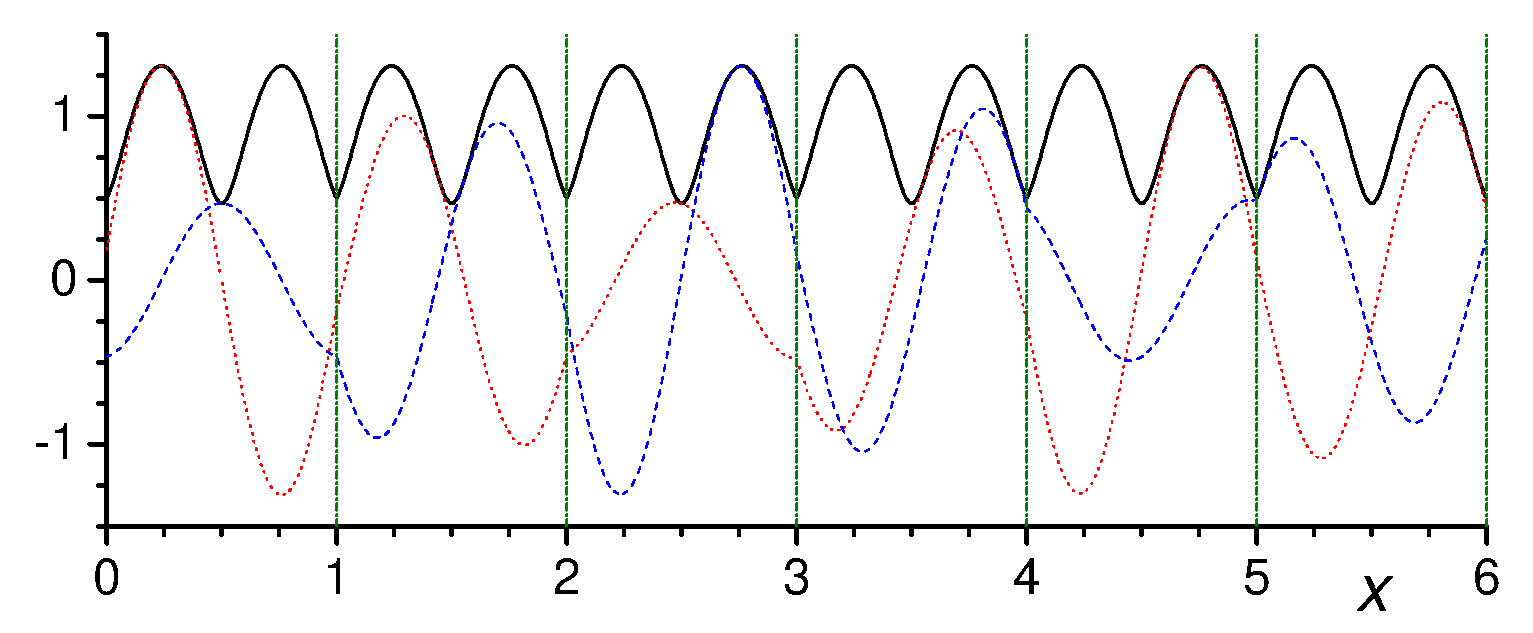
\epsfig{file=psi10_6.eps,width=\linewidth}
            \end{subfigure}
            \scaption{
                Vlnové funkce $\psi_{q}(x)$ normalizované na intervalu $(0,a)$ pro $a=1$, dvě hodnoty $K$ a nejnižší čtyři povolené pásy. 
                Hodnoty $q>0$ leží v 1. Brillouinově zóně.
                Modrá čárkovaná čára -- reálná část, červená tečkovaná čára -- imaginární část, černá čára -- absolutní hodnota.
                Zelené čerchované čáry odpovídají místům, v nichž leží $\delta$-funkce potenciálu.
                Odpovídající energie a hodnoty kvazihybnosti $q$ jsou vyznačeny v obrázku~\ref{fig:DiracCombBands}.
            }
            \label{fig:DiracCombWaveFunctions}
        \end{figure}

        \begin{figure}[!htbp]
            \begin{subfigure}{0.49\linewidth}
                \centering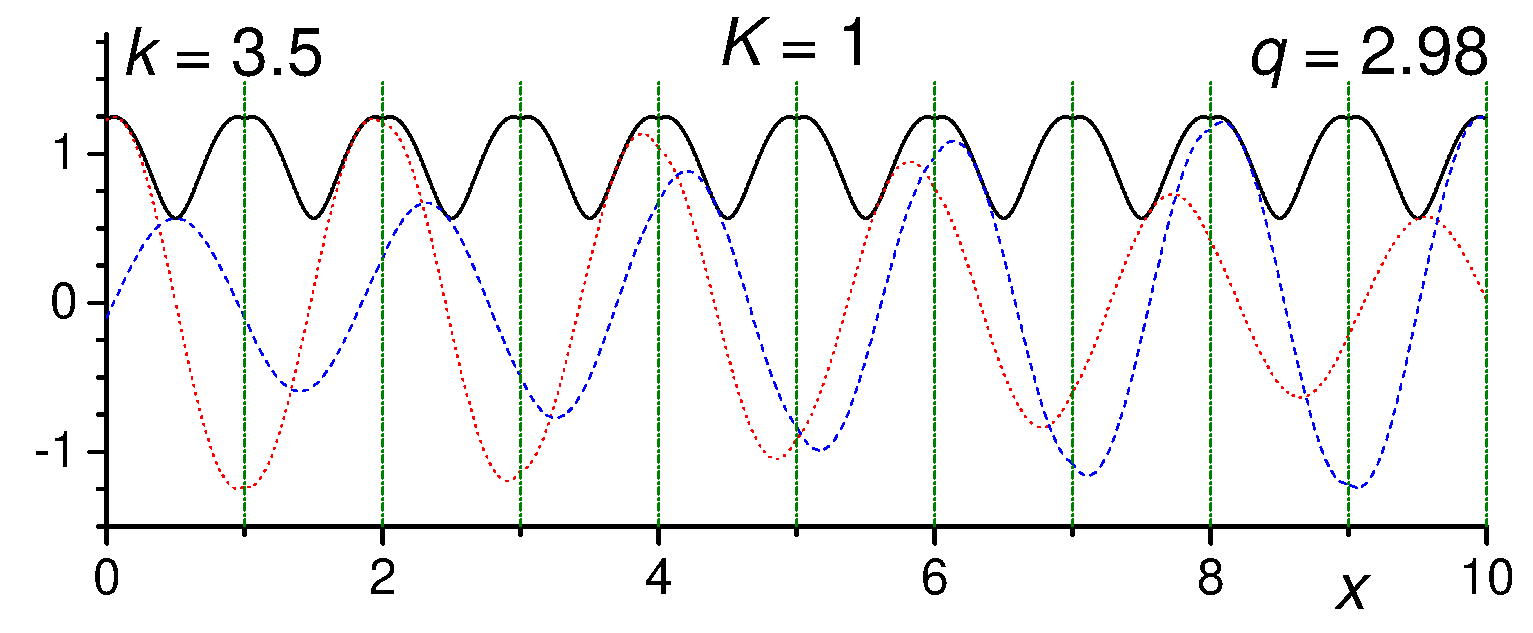
\epsfig{file=psi1s.eps,width=\linewidth}
            \end{subfigure}
            \hfill
            \begin{subfigure}{0.49\linewidth}
                \centering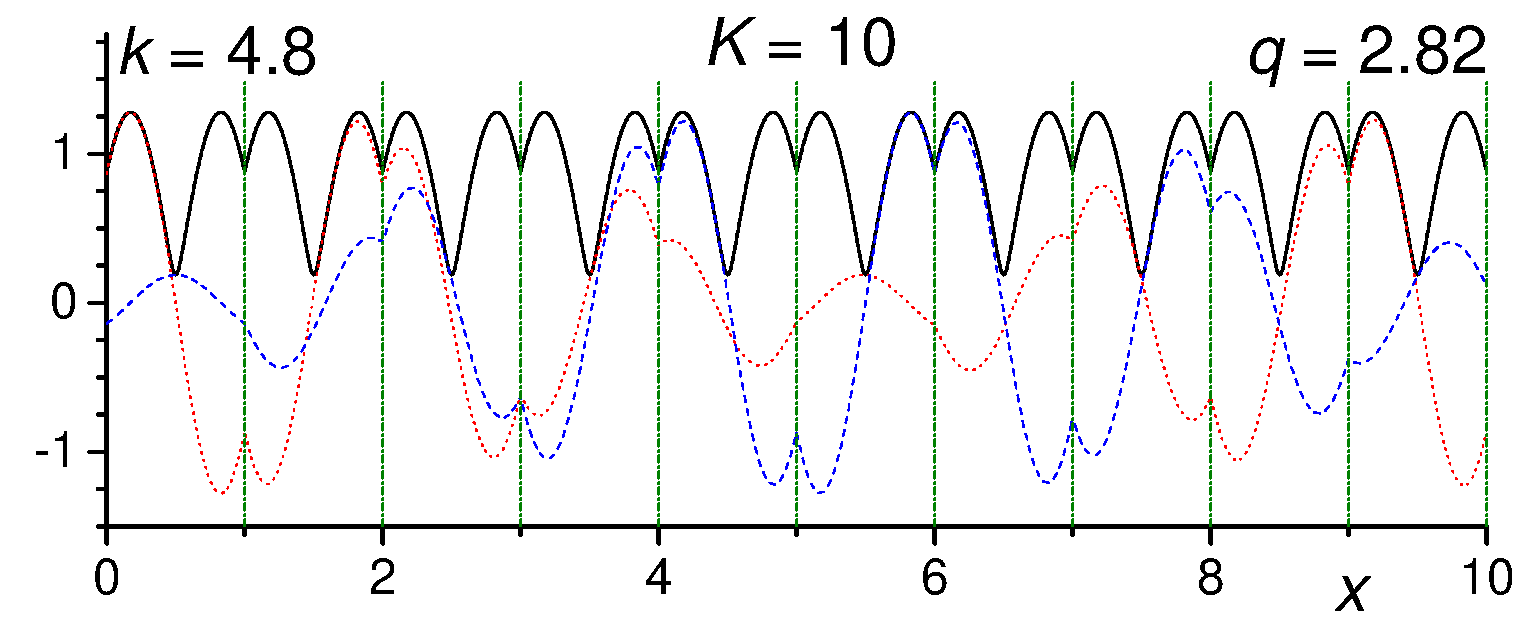
\epsfig{file=psi10s.eps,width=\linewidth}
            \end{subfigure}
            \begin{subfigure}{0.49\linewidth}
                \centering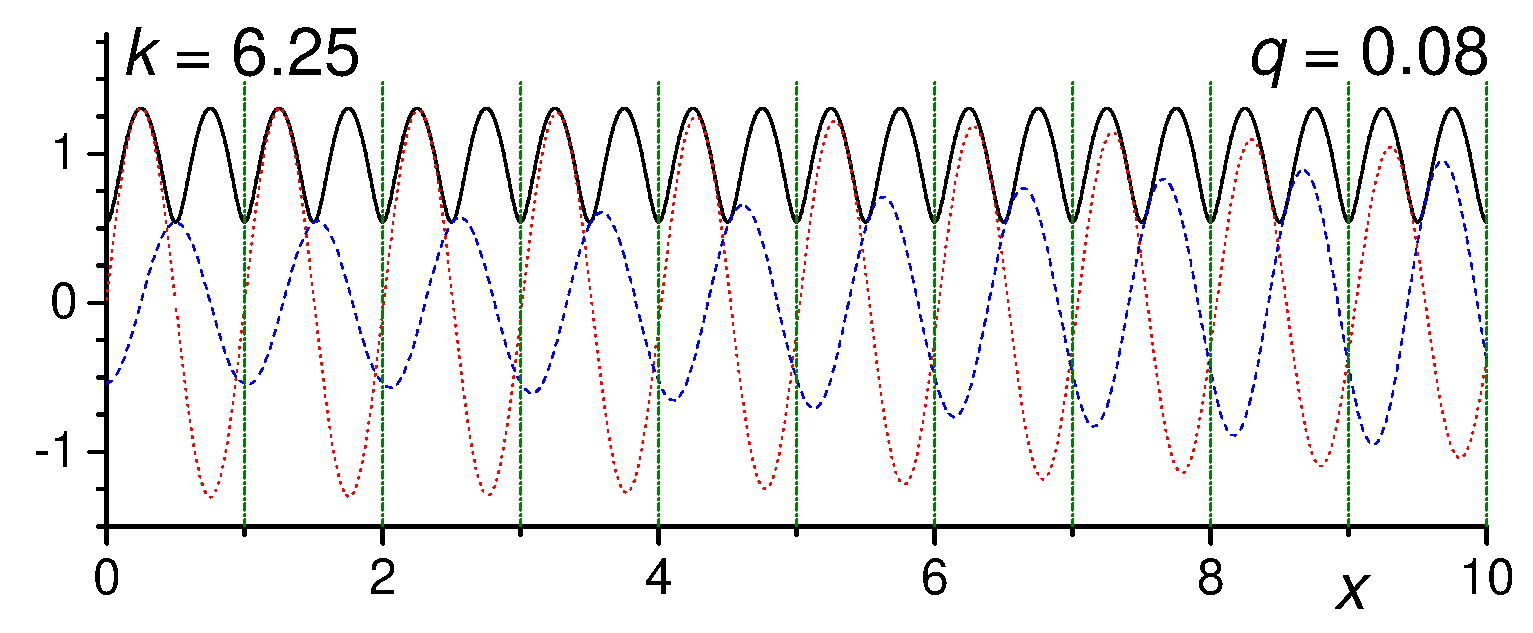
\epsfig{file=psi1e.eps,width=\linewidth}
            \end{subfigure}
            \hfill
            \begin{subfigure}{0.49\linewidth}
                \centering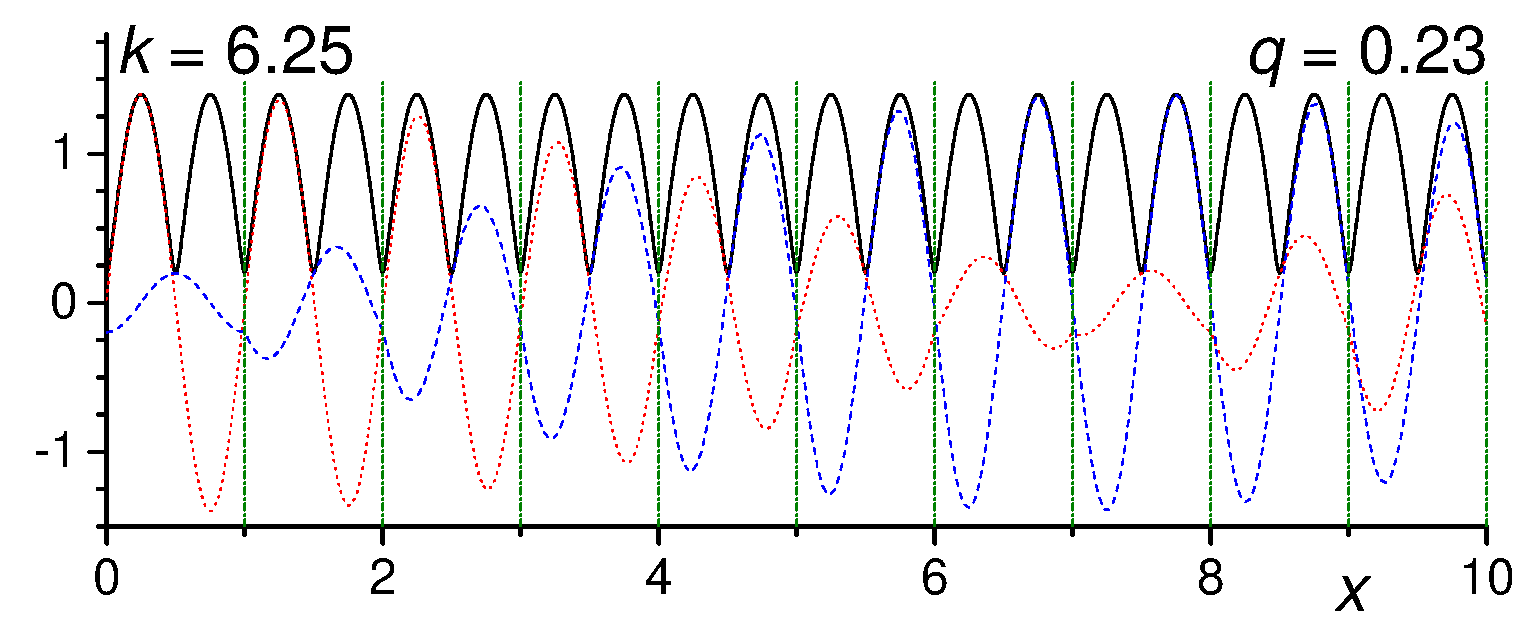
\epsfig{file=psi10e.eps,width=\linewidth}
            \end{subfigure}
            \scaption{
                Totéž jako v obrázku~\ref{fig:DiracCombWaveFunctions}, jen pro vlnové funkce z krajů 2. pásu.	
            }
            \label{fig:DiracCombWaveFunctions2Band}
        \end{figure}

        \begin{figure}[!htbp]
            \begin{subfigure}{0.49\linewidth}
                \centering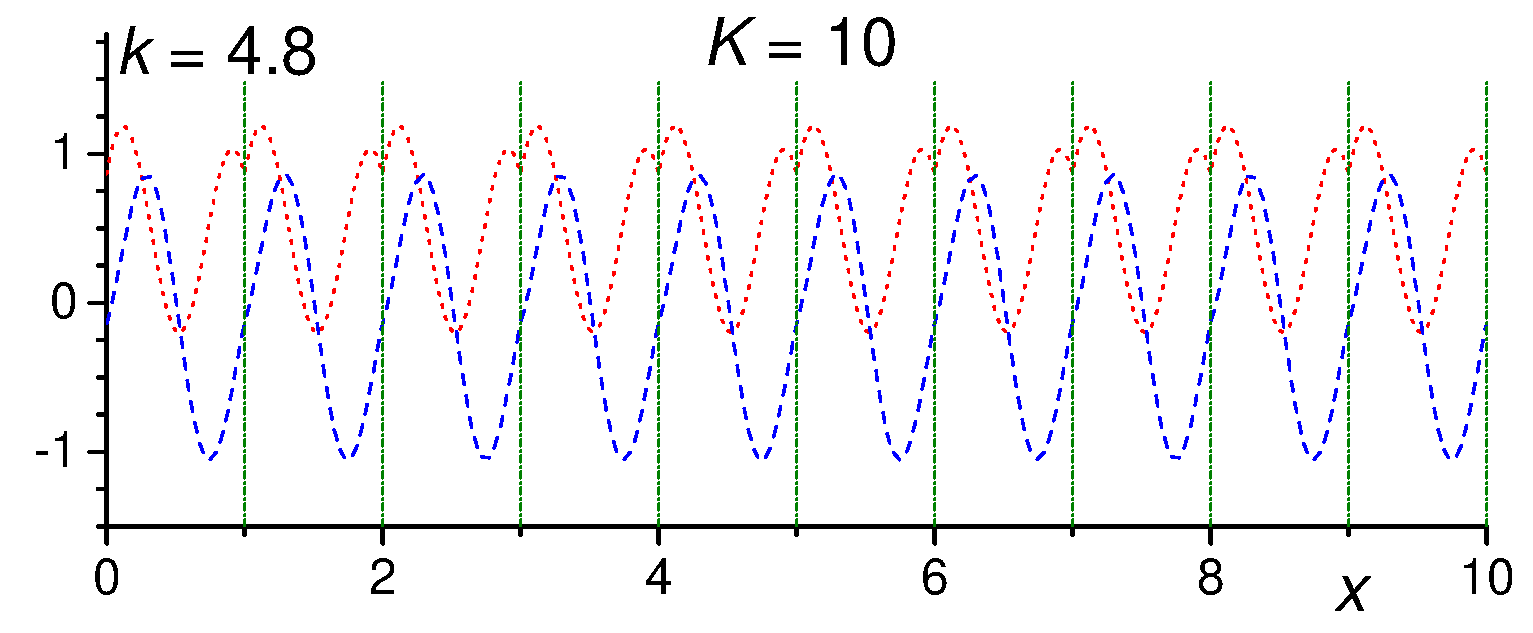
\epsfig{file=us.eps,width=\linewidth}
            \end{subfigure}
            \hfill
            \begin{subfigure}{0.49\linewidth}
                \centering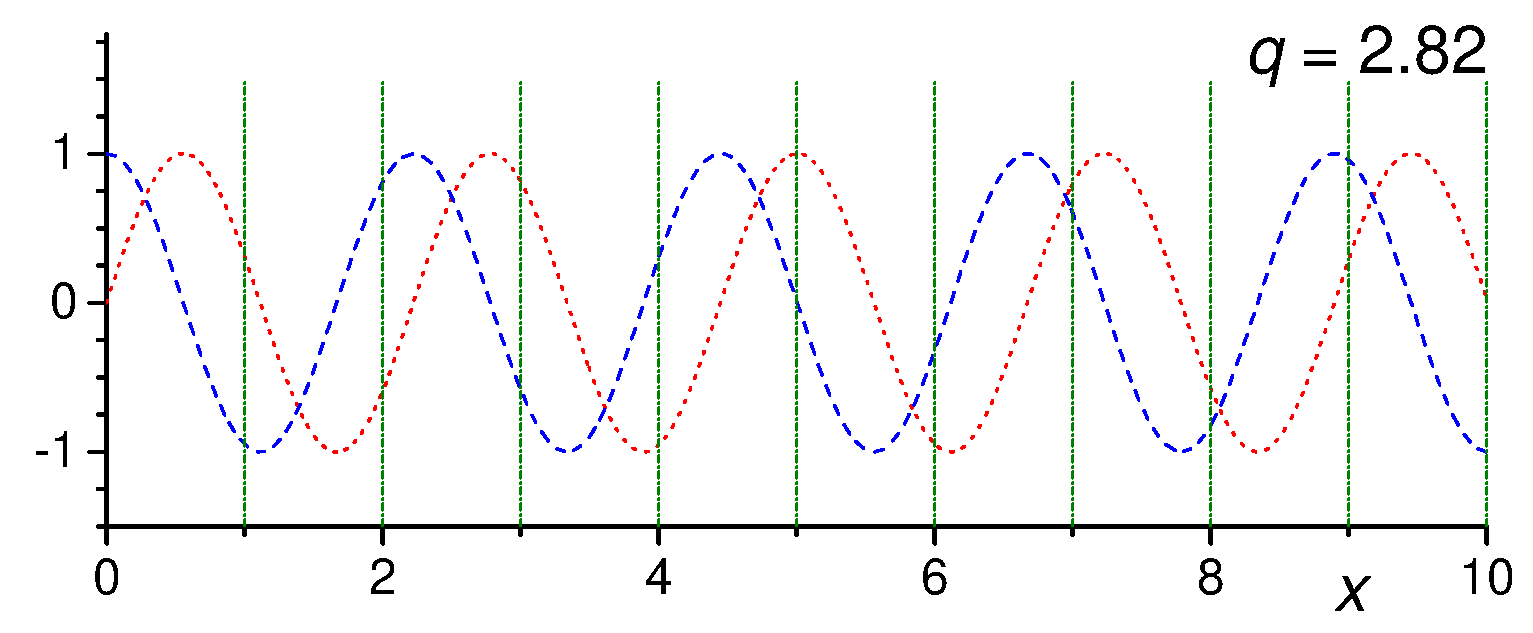
\epsfig{file=uqs.eps,width=\linewidth}
            \end{subfigure}
            \begin{subfigure}{0.49\linewidth}
                \centering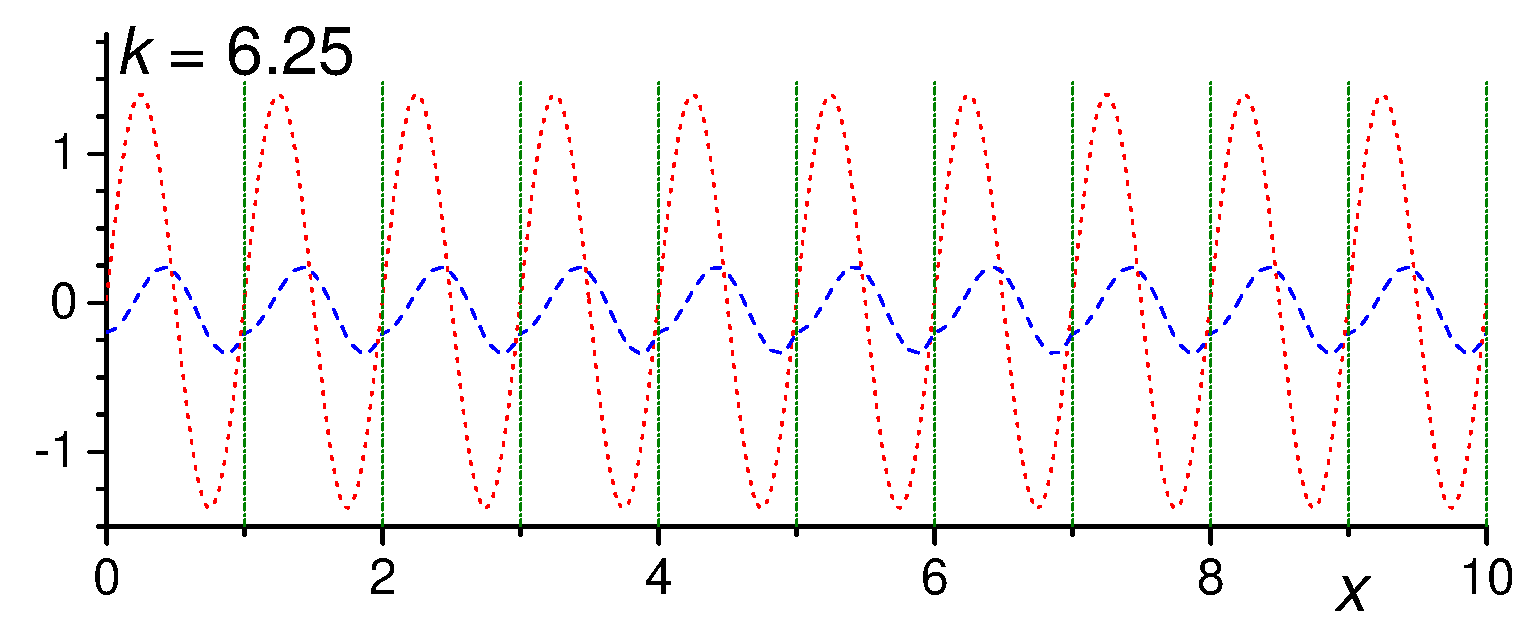
\epsfig{file=ue.eps,width=\linewidth}
            \end{subfigure}
            \hfill
            \begin{subfigure}{0.49\linewidth}
                \centering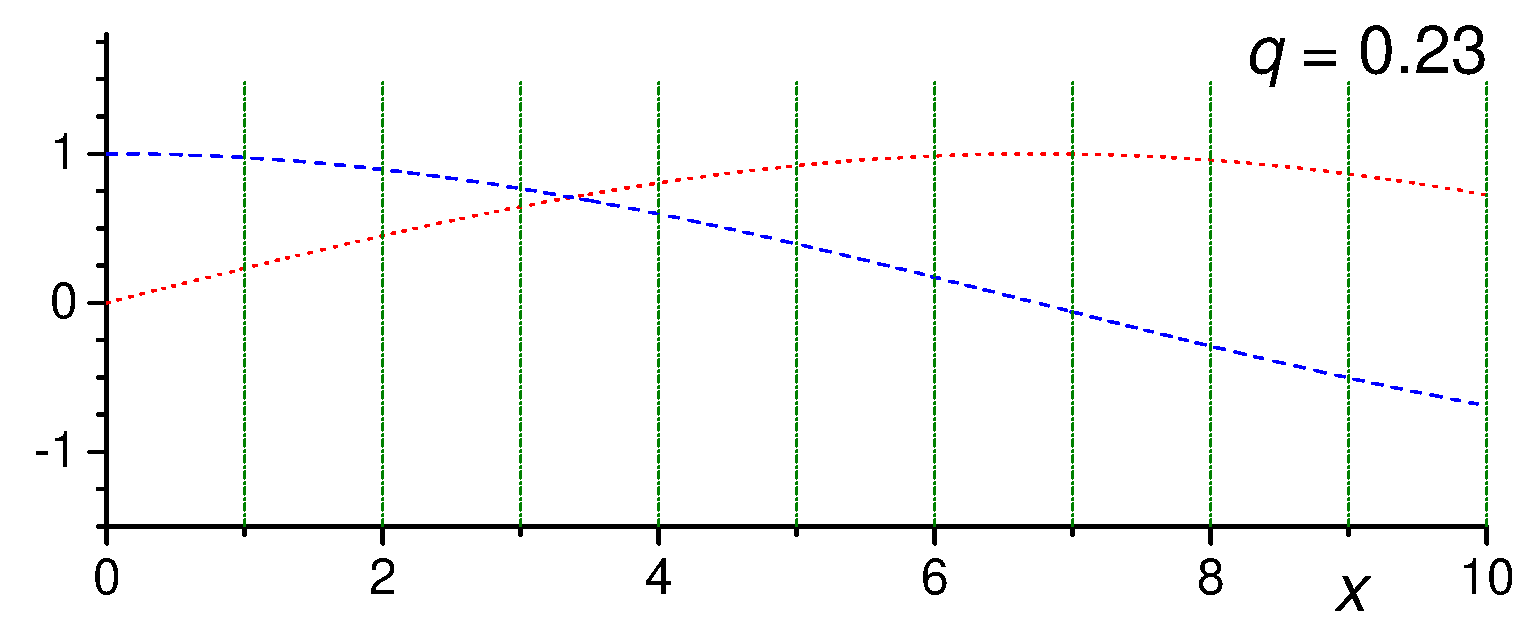
\epsfig{file=uqe.eps,width=\linewidth}
            \end{subfigure}
            \scaption{
                Periodická část vlnové funkce $u_{q}(x)$ (vlevo) a Blochova vlna $\e^{\im q x}$ (vpravo).
                Modrá čárkovaná čára -- reálná část, červená tečkovaná čára -- imaginární část.
                Pronásobení sloupců mezi sebou dá vlnové funkce z pravého sloupce obrázku~\ref{fig:DiracCombWaveFunctions2Band}.
            }
            \label{fig:DiracCombBlochWave}
        \end{figure}

        Podobně lze vyjádřit
        \begin{align}
            1&=2a\abs{A}^{2}\frac{1-\cos{qa}\cos{ka}+\frac{2}{Ka}\left(\cos{qa}-\cos{ka}\right)^{2}}{1-\cos{(q+k)a}},
        \end{align}
        takže normalizační konstanty jsou
        \begin{subequations}
            \begin{align}
                A&=s\sqrt{\frac{1}{2a}\frac{1-\cos{(q+k)a}}{1-\cos{qa}\cos{ka}+\frac{2}{Ka}\left(\cos{qa}-\cos{ka}\right)^{2}}}\e^{-\im\frac{ka}{2}},\\
                B&=\sqrt{\frac{1}{2a}\frac{1-\cos{(q-k)a}}{1-\cos{qa}\cos{ka}+\frac{2}{Ka}\left(\cos{qa}-\cos{ka}\right)^{2}}}\e^{\im\frac{ka}{2}},\\
                s&=\sign\left(\cos{qa}-\cos{ka}\right)
            \end{align}
        \end{subequations}
        (komplexní fáze se rozdělila stejným dílem mezi $A$ a $B$; je nutné udržet znaménko mezi $A$ a $B$).
        Získaný výsledek je v souladu s rovnicí (9) článku~\cite{Kronig1931}.
        
        Vlnová funkce normalizovaná na interval $(0,a)$ je tedy
        \begin{align}
            \psi_{q}(x)
                &=\frac{\e^{\im qna}}{\sqrt{2a}}\frac{1}{\sqrt{1-\cos{qa}\cos{ka}+\frac{2}{Ka}\left(\cos{qa}-\cos{ka}\right)^{2}}}\\
                &\qquad*\left[s\sqrt{1-\cos{(q+k)a}}\e^{\im k\left(x-na-\frac{a}{2}\right)}+\sqrt{1-\cos{(q-k)a}}\e^{-\im k\left(x-na-\frac{a}{2}\right)}\right].\nonumber
        \end{align}
        Několik příkladů vlnových funkcí je na obrázcích~\ref{fig:DiracCombWaveFunctions} a~\ref{fig:DiracCombWaveFunctions2Band}.
        Vlnová funkce rozložená na periodickou část a Blochovu vlnu je na obrázku~\ref{fig:DiracCombBlochWave}.
        Je vidět, že pro slabou interakci a střed pásu je pravděpodobnost nalezení částice prakticky konstantní (obrázek~\ref{fig:DiracCombWaveFunctions}, 1. sloupec, 3.--5. řádek).
        Naopak na krajích pásu nebo pro silnější interakci hustota pravděpodobnosti více osciluje (obrázek~\ref{fig:DiracCombWaveFunctions}, 2. sloupec, a obrázek~\ref{fig:DiracCombWaveFunctions2Band}).

    \item
        \begin{figure}[!htbp]
            \begin{subfigure}{0.49\linewidth}
                \centering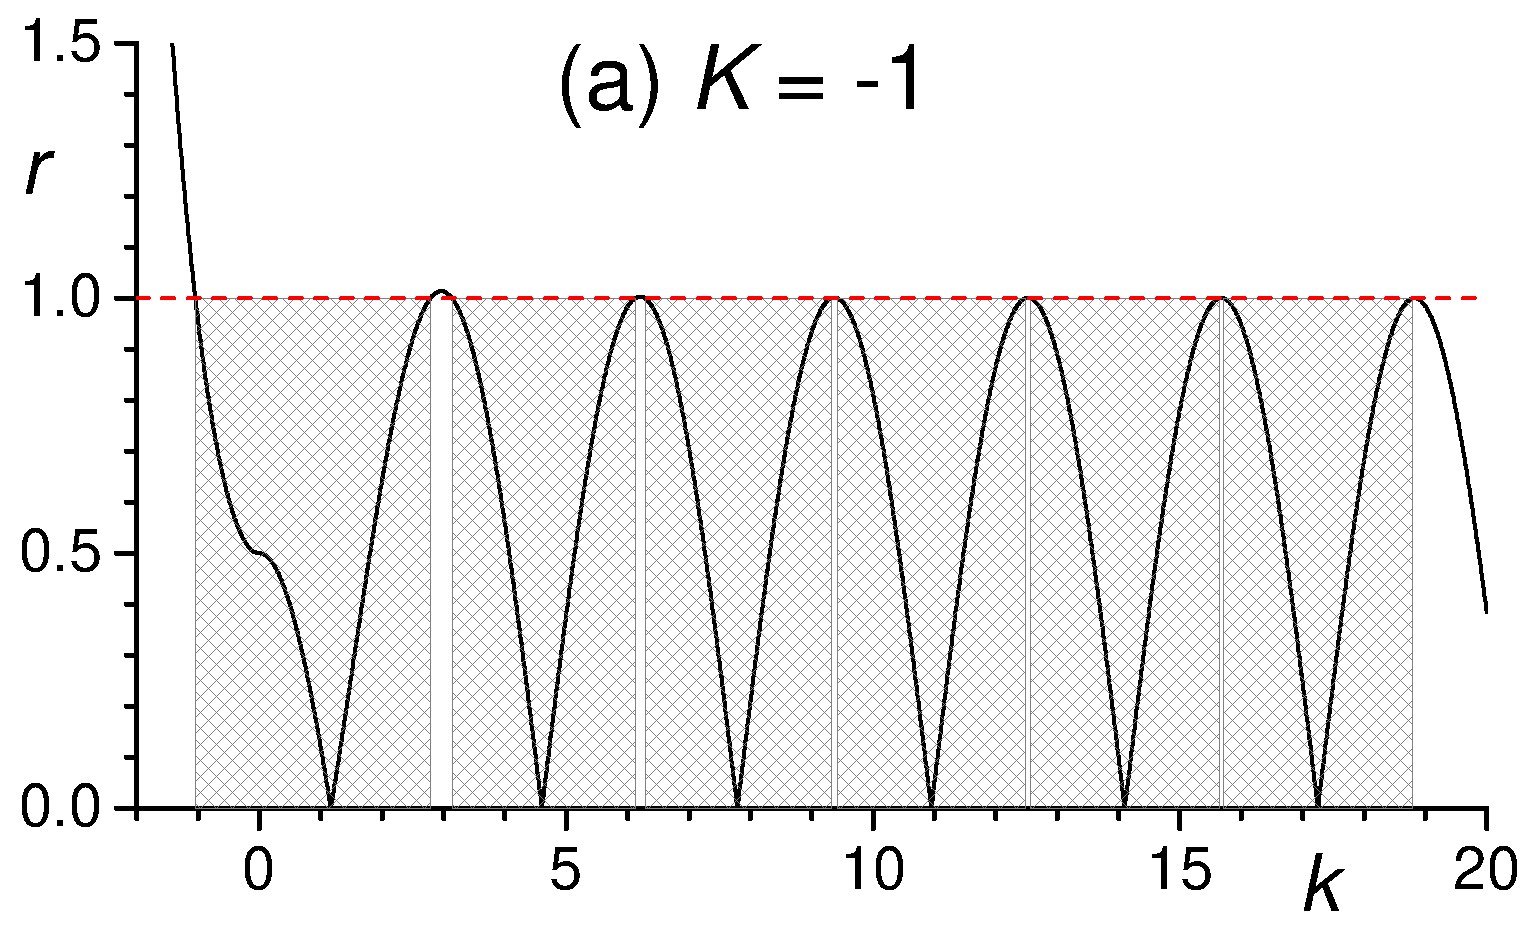
\epsfig{file=bandf1n.eps,width=\linewidth}
            \end{subfigure}
            \hfill
            \begin{subfigure}{0.49\linewidth}
                \centering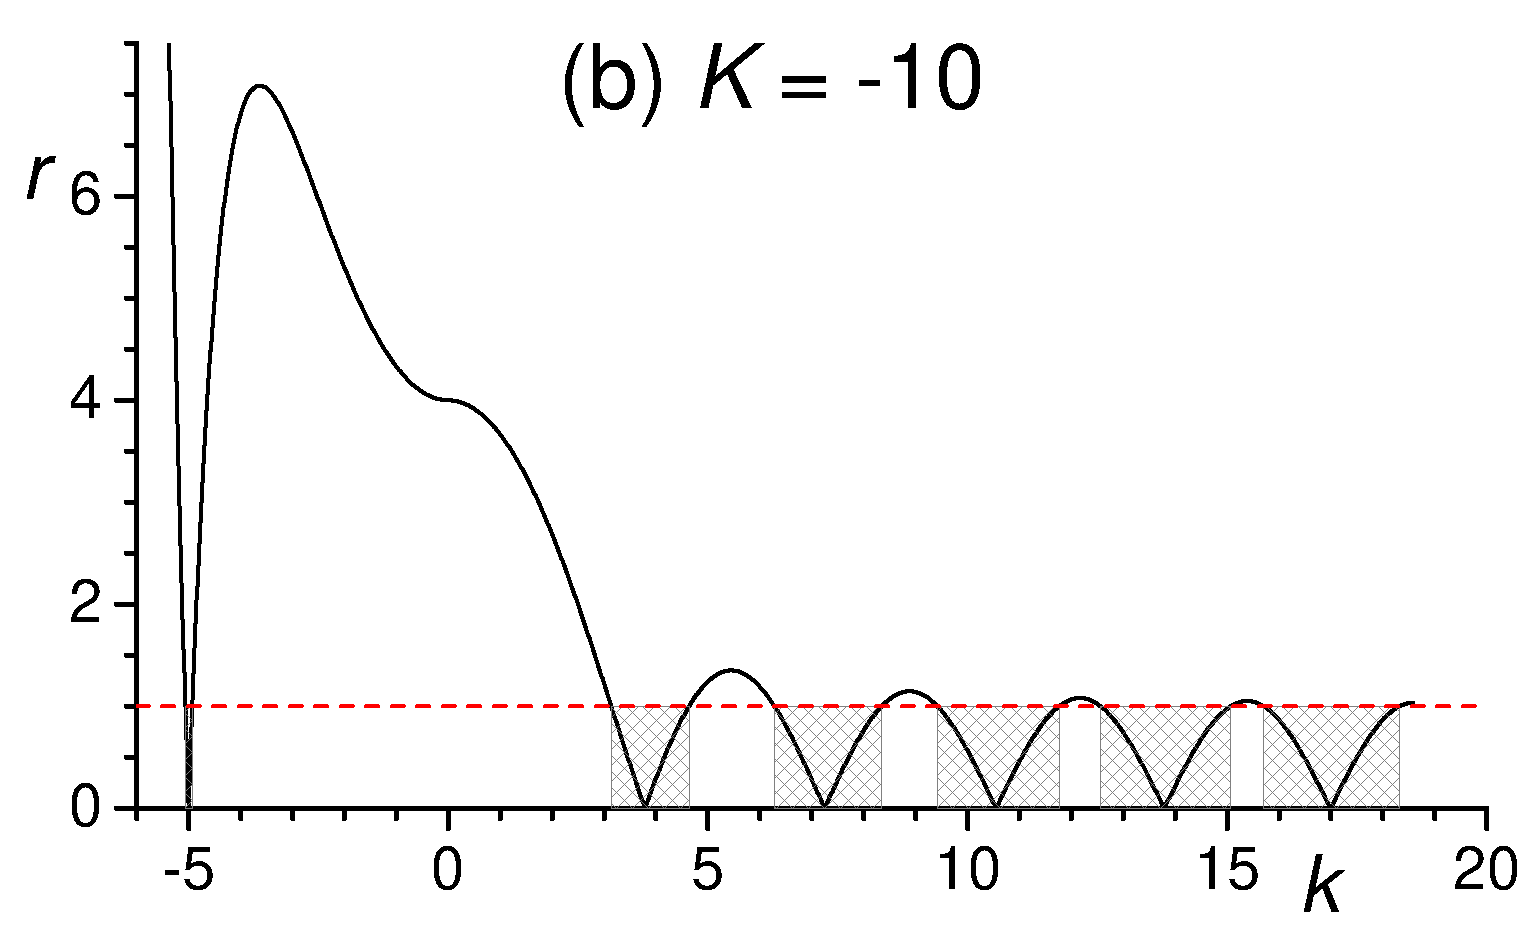
\epsfig{file=bandf10n.eps,width=\linewidth}
            \end{subfigure}
            \scaption{
                Funkce $r$ (černá čára) pro dvě záporné hodnoty parametru $K$ a mřížkovou konstantu $a=1$.
                Pásy, v nichž lze vyřešit rovnici~\eqref{eq:DiracCombBand} (pro $E<0$) a~\eqref{eq:DiracCombBandNegative} (pro $E>0$) jsou vyznačeny šrafováním.
            }
            \label{fig:DiracCombBandConditionNegative}
        \end{figure}

        \begin{figure}[!htbp]
            \begin{subfigure}{0.49\linewidth}
                \centering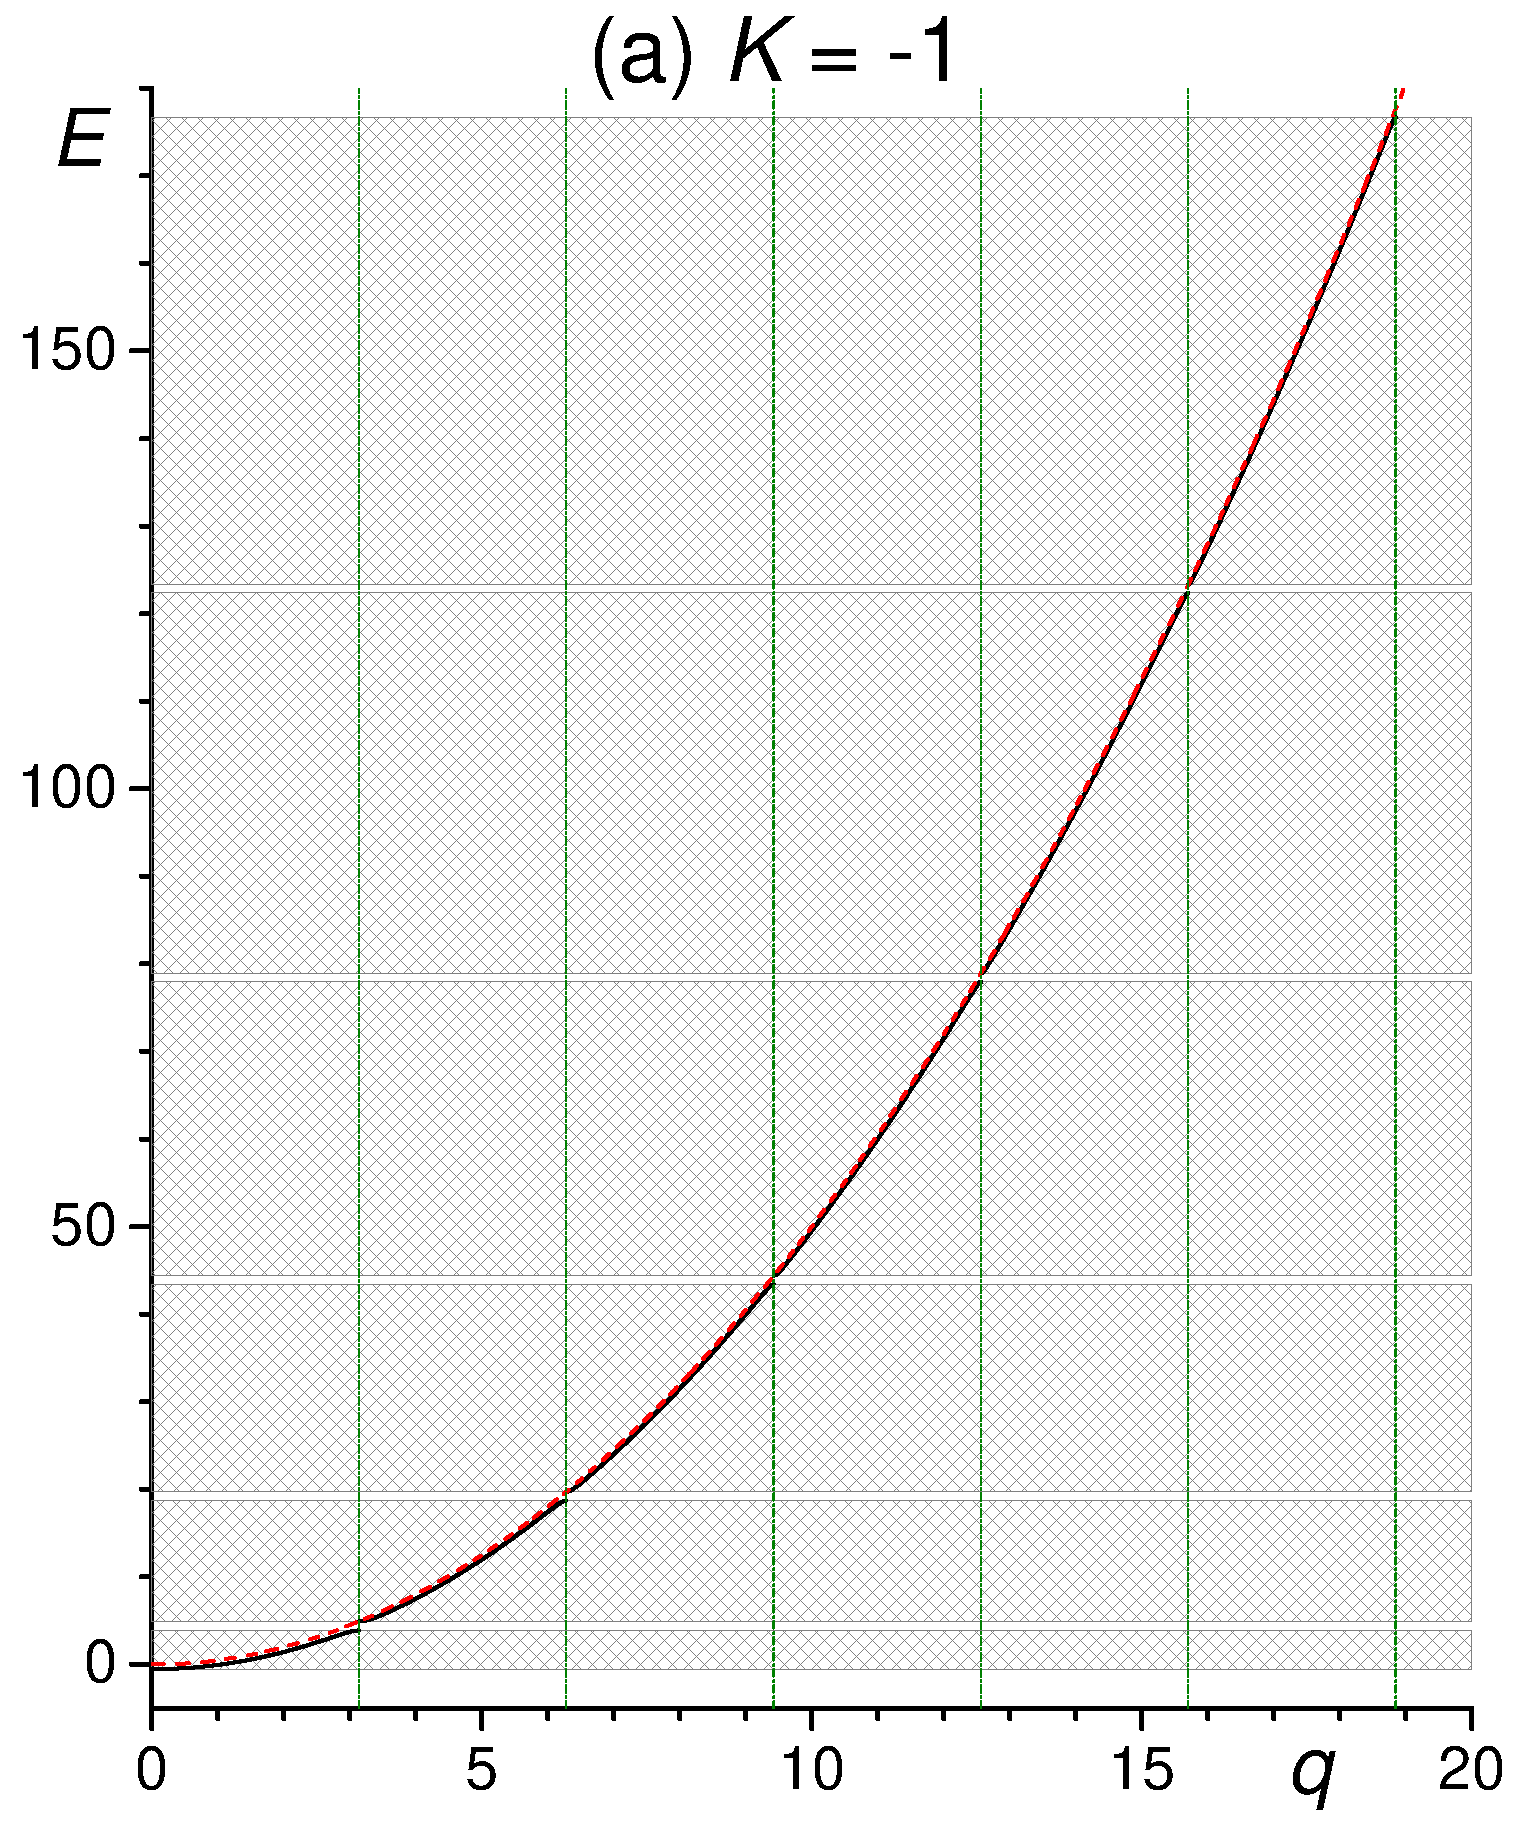
\epsfig{file=bands1n.eps,width=\linewidth}
            \end{subfigure}
            \hfill
            \begin{subfigure}{0.49\linewidth}
                \centering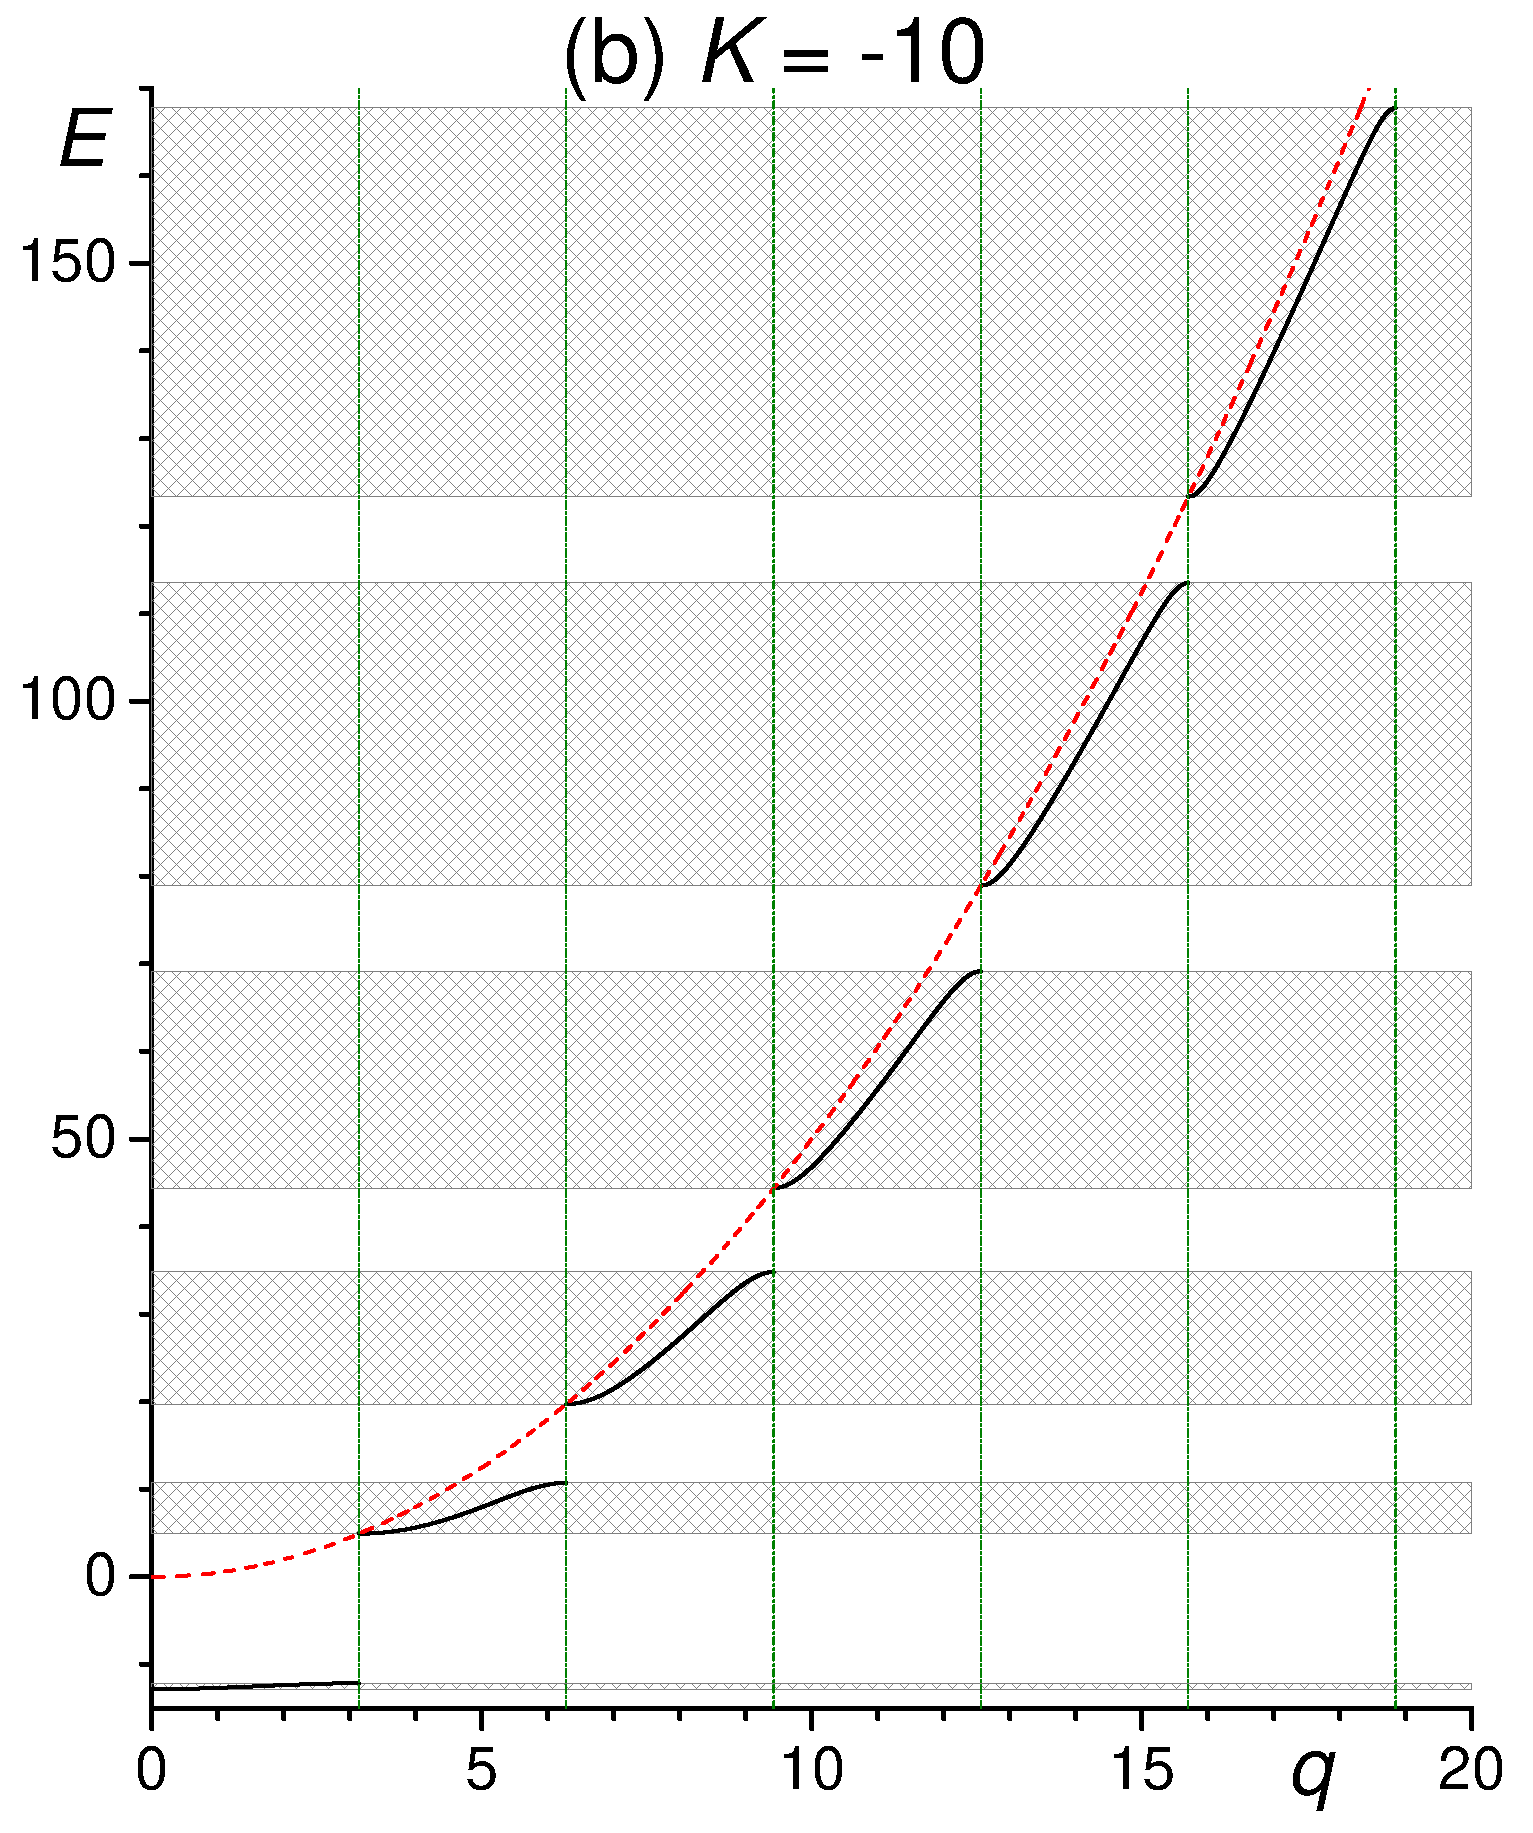
\epsfig{file=bands10n.eps,width=\linewidth}
            \end{subfigure}
            \begin{subfigure}{0.49\linewidth}
                \centering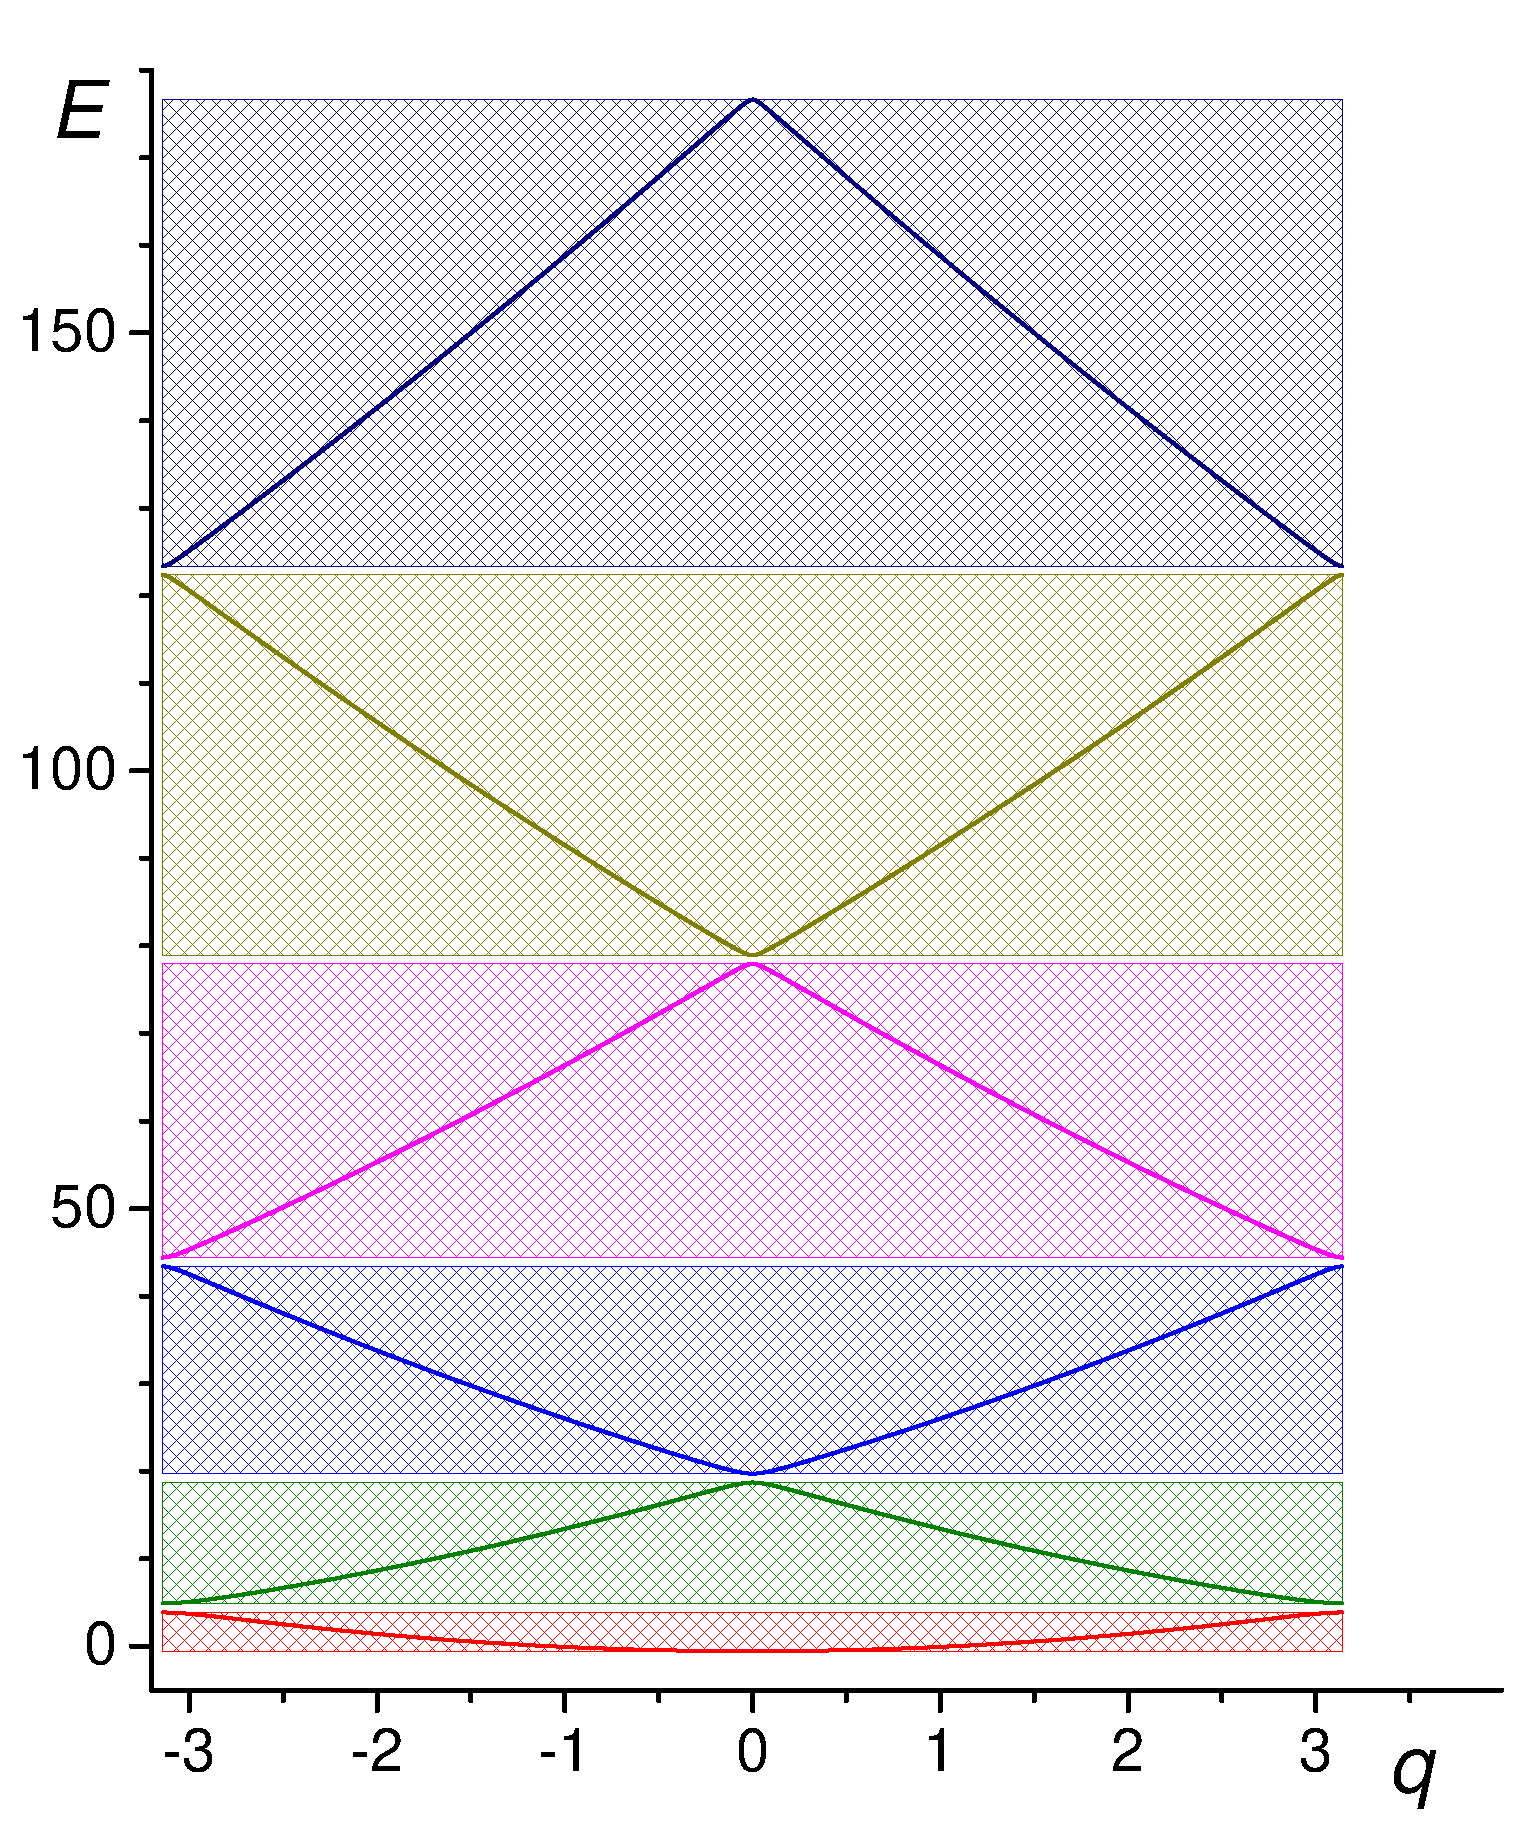
\epsfig{file=Brillouin1n.eps,width=\linewidth}
            \end{subfigure}
            \hfill
            \begin{subfigure}{0.49\linewidth}
                \centering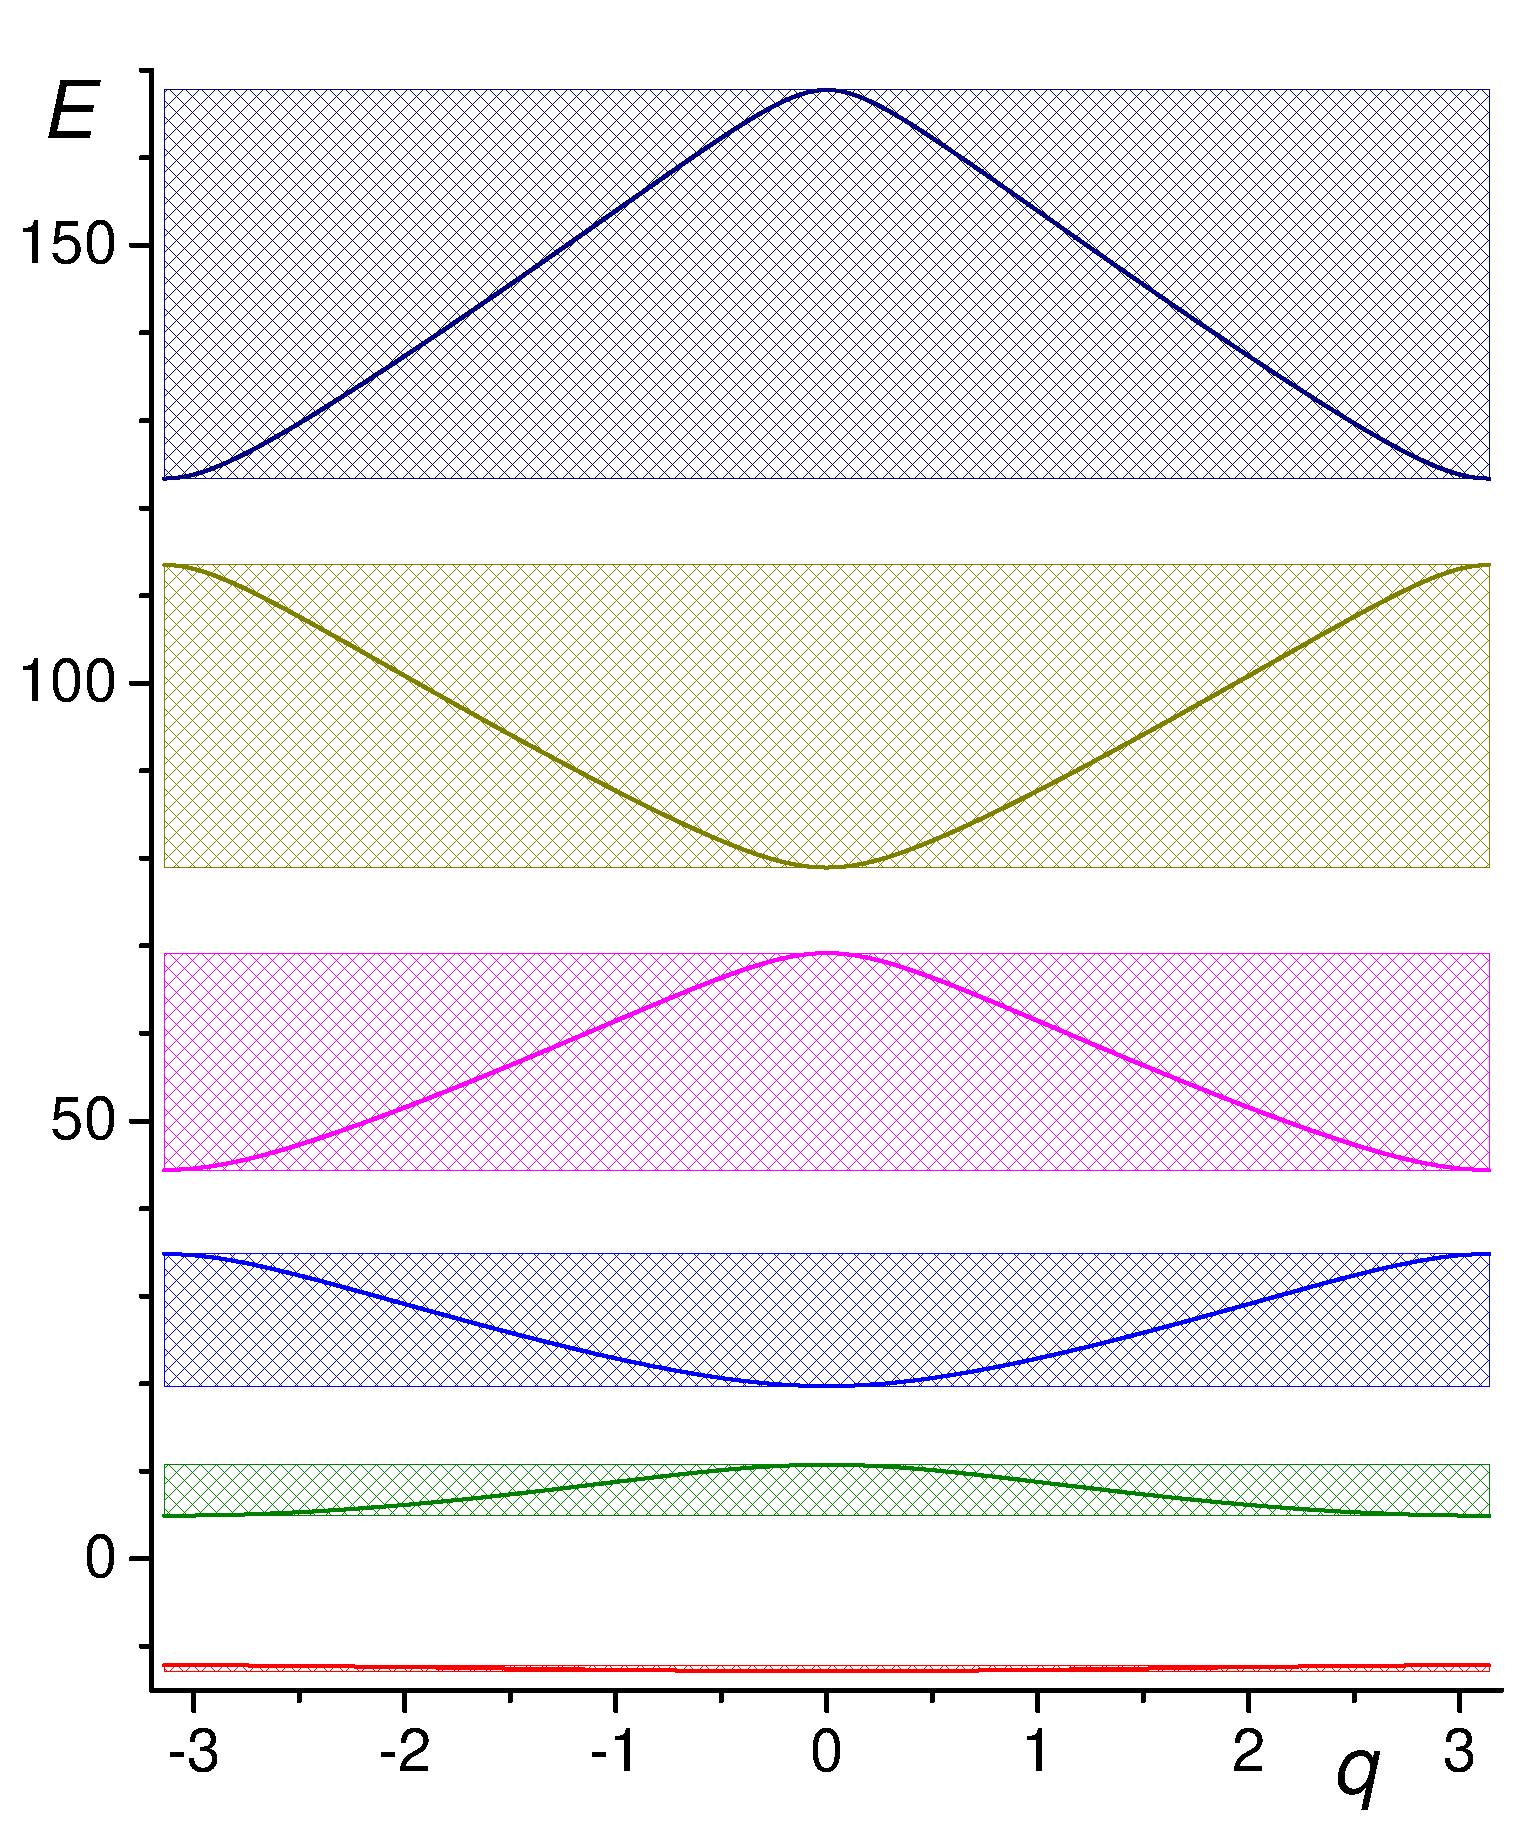
\epsfig{file=Brillouin10n.eps,width=\linewidth}
            \end{subfigure}
            \scaption{
                \emph{1. řádek:} Disperzní relace v konvenci~\eqref{eq:DiracCombBandUnique} pro dvě hodnoty $K$ (černá čára).
                Červená čárkovaná čára odpovídá disperzní relaci pro volnou částici $E=\hbar^{2}q^{2}/(2M)$.
                Svislé zelené čerchované čáry vyznačují horní hranice pásů~\eqref{eq:DiracCombBandTop}.				
                Šrafováním jsou znázorněny povolené pásy.				
                \emph{2. řádek:}
                Disperzní relace pro 1. Brillouinovu zónu~\eqref{eq:Brillouin}.
                Jednotlivé pásy jsou znázorněny odlišnými barvami.
            }
            \label{fig:DiracCombBandsNegative}
        \end{figure}
        
        \begin{figure}[!htbp]
            \begin{subfigure}{0.49\linewidth}
                \centering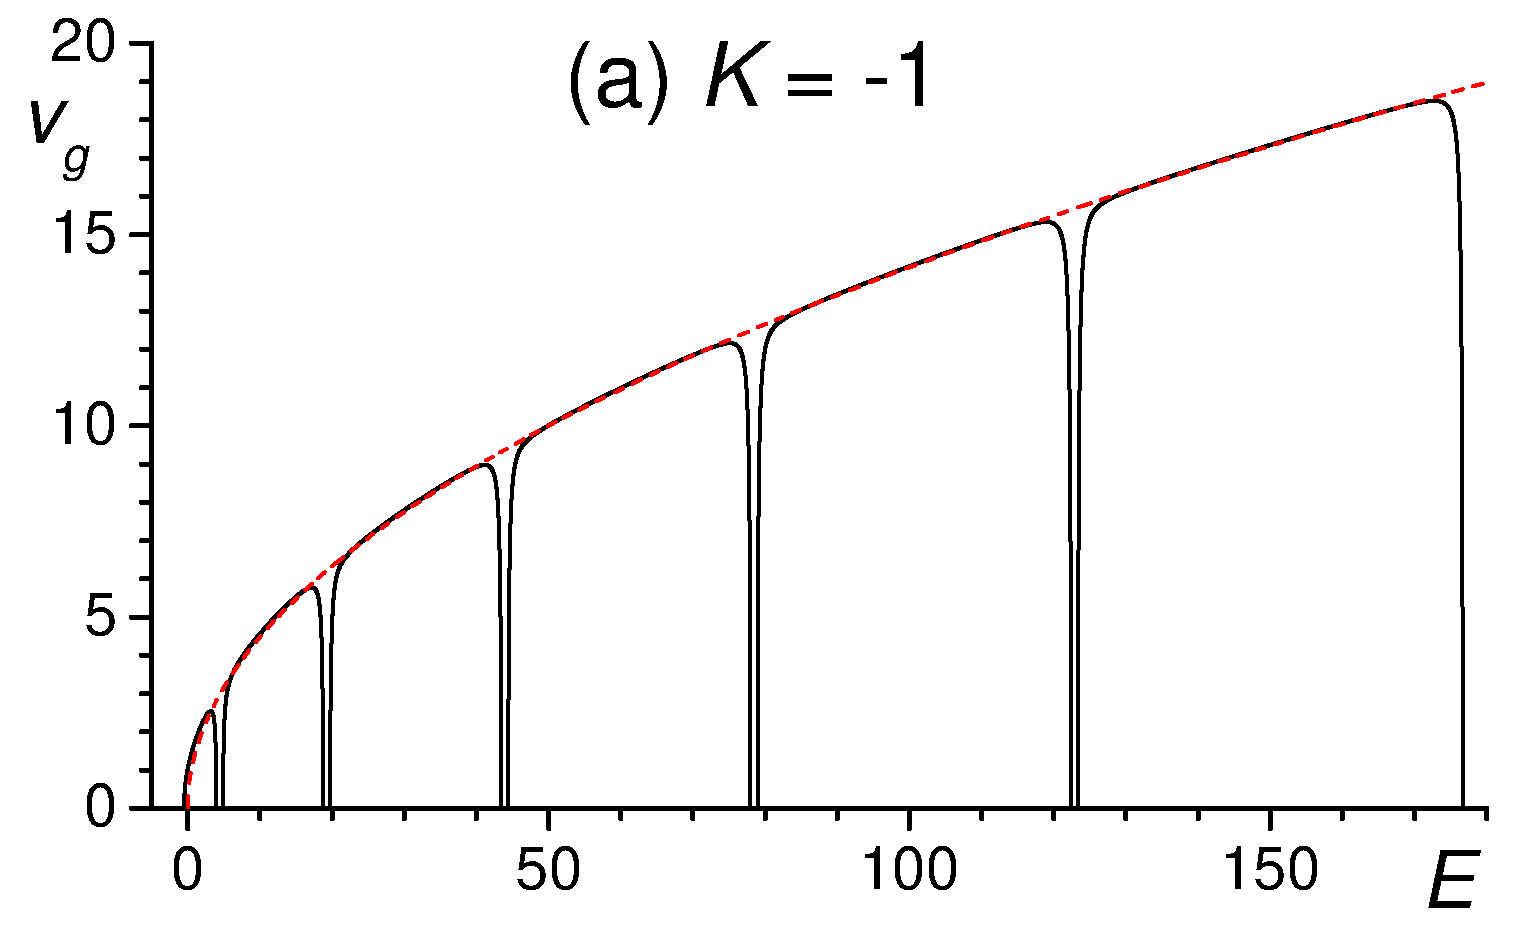
\epsfig{file=vgE1n.eps,width=\linewidth}
            \end{subfigure}
            \hfill
            \begin{subfigure}{0.49\linewidth}
                \centering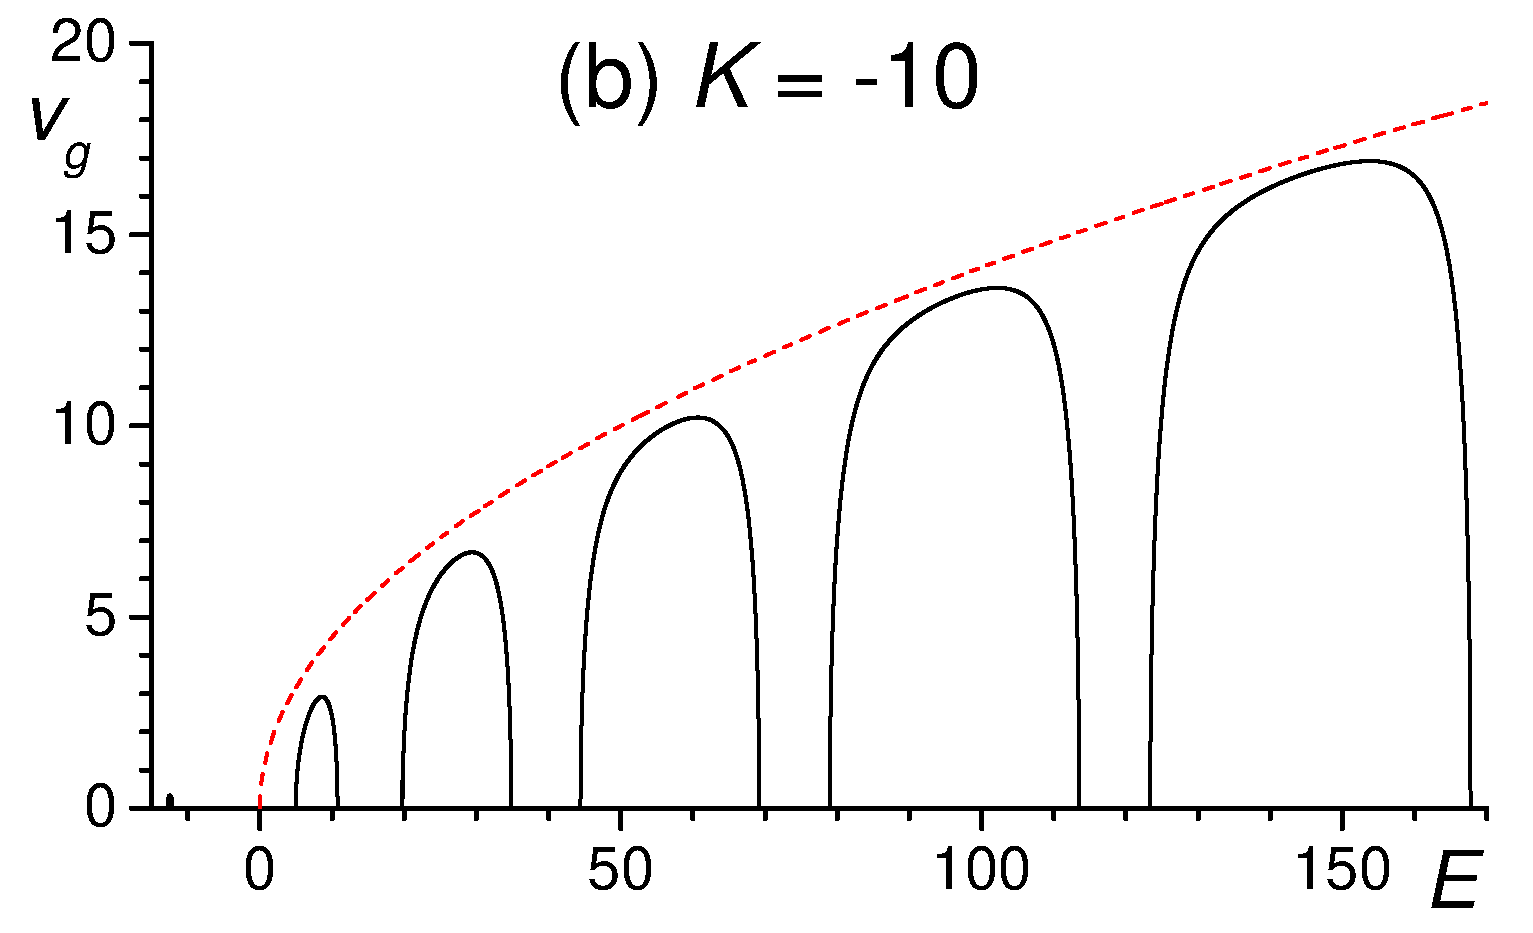
\epsfig{file=vgE10n.eps,width=\linewidth}
            \end{subfigure}
            \begin{subfigure}{0.49\linewidth}
                \centering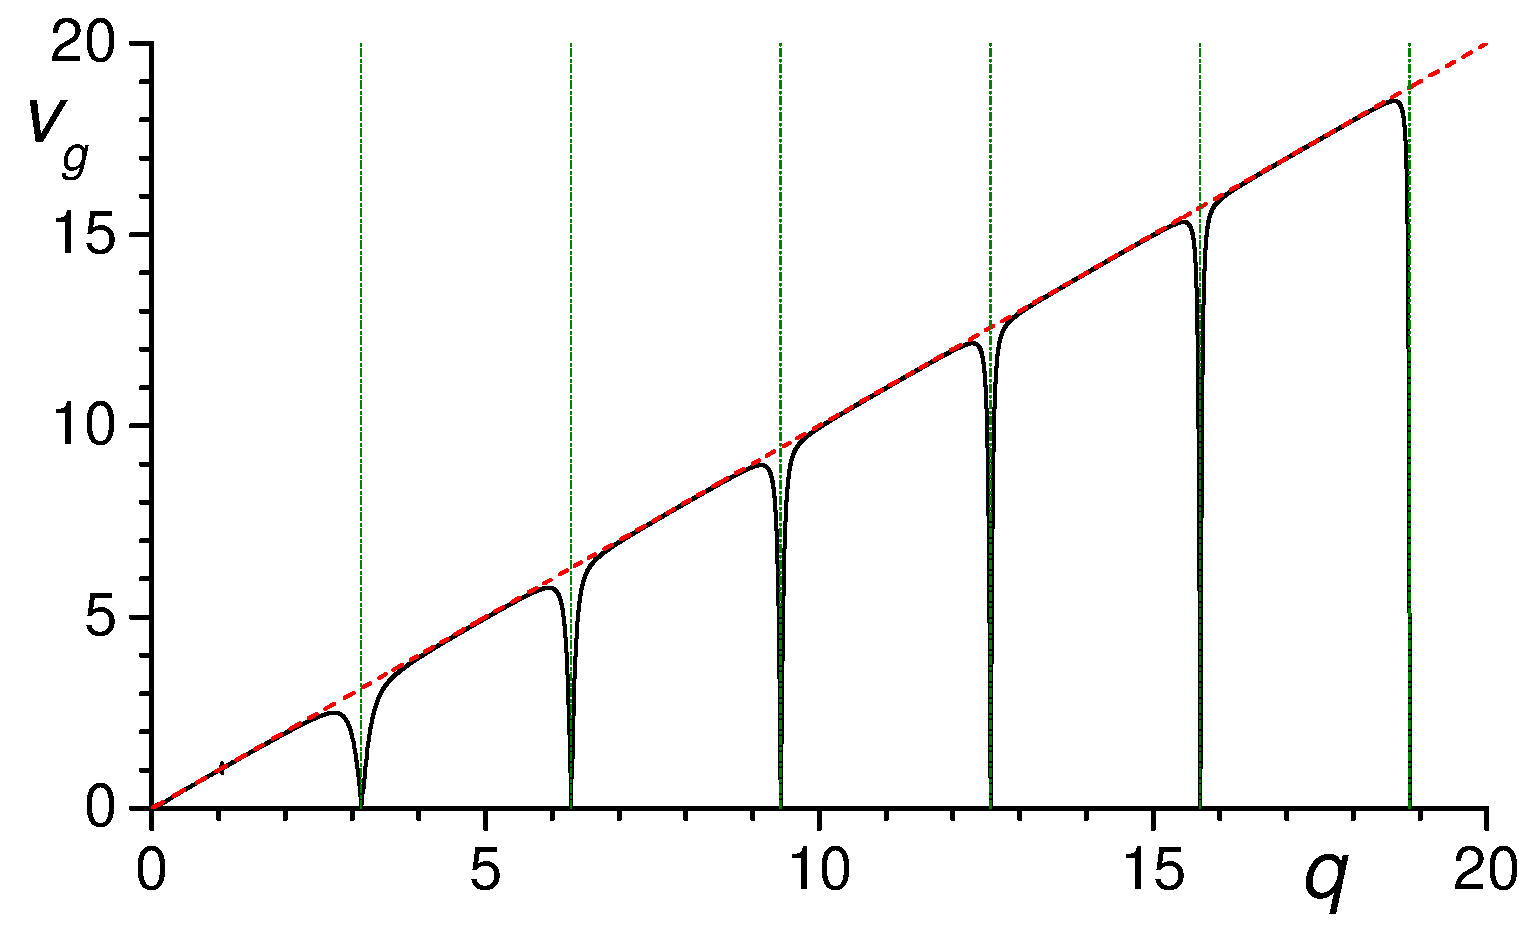
\epsfig{file=vgq1n.eps,width=\linewidth}
            \end{subfigure}
            \hfill
            \begin{subfigure}{0.49\linewidth}
                \centering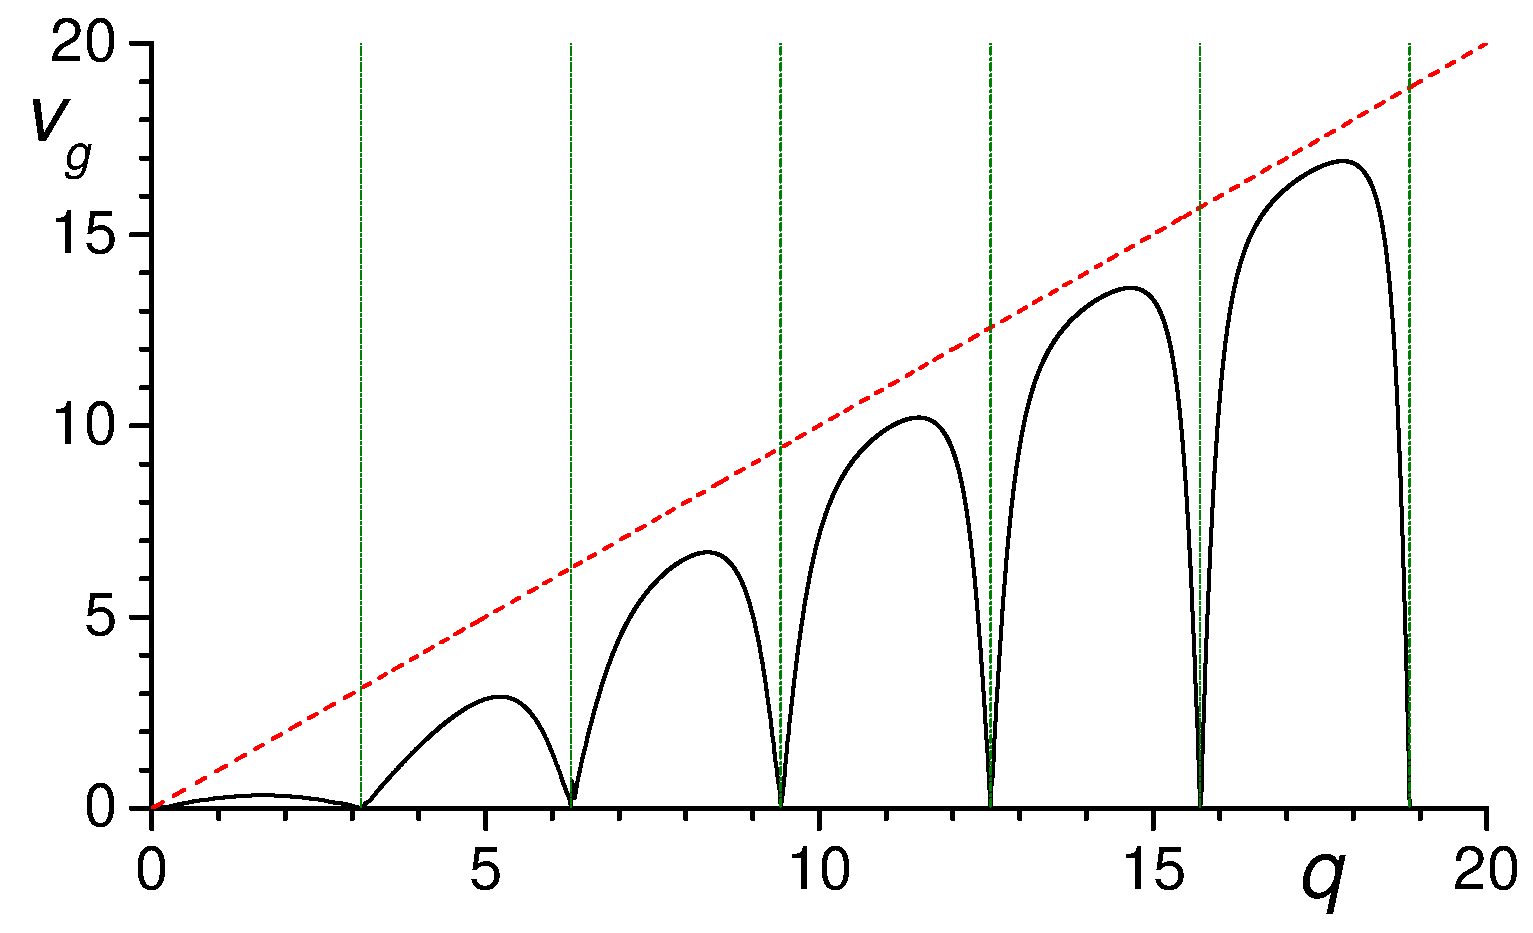
\epsfig{file=vgq10n.eps,width=\linewidth}
            \end{subfigure}
            \scaption{
                Grupová rychlost~\eqref{eq:DiracCombGroupVelocity} v závislosti na energii (1. řádek) a na kvazihybnosti (2. řádek).
                Ve 2. řádku jsou hranice pásů $q=\pi n$ znázorněny svislými zelenými čerchovanými čarami.
                Červená čárkovaná čára odpovídá rychosti pro volnou částici $E=\hbar q/M$.
            }
            \label{fig:DiracCombGroupVelocityNegative}
        \end{figure}

        V souladu s případem izolovaných $\delta$ jam (viz příklady~\ref{sec:Delta} a~\ref{sec:DoubleDelta}) se označí
        \begin{equation}
            \kappa=\sqrt{-\frac{2ME}{\hbar^{2}}}.
        \end{equation}
        Formálně tedy platí $k=\im\kappa$, čehož lze využít v rovnici~\eqref{eq:DiracCombBand} a dojít k podmínce
        \begin{equation}\label{eq:DiracCombBandNegative}
            \boxed{\cos{qa}=\cosh{\kappa a}+\frac{K}{2\kappa}\sinh{\kappa a}}.
        \end{equation}
        Pro $K\in(-\frac{4}{a},0)$ leží nulová energie v nejnižším pásu.
        Pokud $K<-\frac{4}{a}$, první povolený pás se nachází na enegii $E<0$ a na energii $E=0$ je zakázaný pás.
        
        V analogii s obrázky~\ref{fig:DiracCombBands}---\ref{fig:DiracCombGroupVelocity} je na obrázcích~\ref{fig:DiracCombBandsNegative}---\ref{fig:DiracCombGroupVelocityNegative} zobrazen průběh veličiny $r$, disperzní relace $E(q)$ v konvenci~\eqref{eq:DiracCombBandUnique} a v 1. Brillouinově zóně a grupová rychlost pro dvě záporné hodnoty síly interakce $K$.

    \end{enumerate}
\end{solution}
